\documentclass{article}
\usepackage{amsmath,amssymb,amsthm,enumitem} % Some standard math packages.
\usepackage{titling} % Enables \setlength{\droptitle}
\usepackage{parskip} % Cleaner paragraph display
\usepackage[margin=1in]{geometry} % Adjusts margins.
\usepackage[utf8]{inputenc} % USe UTF-8 input encoding instead of default ASCII.
\usepackage[]{forest} % Draws trees.
\usepackage{fancyvrb} % Allows Verbatim sections with line numbers and such. Note the capital V.
\usepackage{pgfplots} % For drawing graphs
\usepackage{hyperref} % For hyperlinks
\usepackage{subcaption} % For subfigure environment
\pgfplotsset{compat=1.6}
\newcommand {\todo}[1] {{\textbf{\color{red}#1}}}

\title{CS 584 Research Project \\ \large Portland State University}
\author{ Dylan Laufenberg }
\date{June 5, 2018}

\begin{document}
\maketitle

\paragraph{Project topic} I will implement a variety of data structures that maintain total orders on their data, e.g. 2-3 trees, treaps, and skip lists; I will choose at least one deterministic structure as a reference and at least one randomized data structure for comparison. I will experimentally evaluate the rates of growth of their run times for insertions, searches, and deletions. Based on these data, I will discuss how the performance I observe compares to the predicted asymptotic performance.

\section{Introduction}
This paper aims to illuminate various facets of the relationship between asymptotic complexity and empirical performance of a range of related data structures. The vehicle for this exploration is a series of benchmarks of data structures that perform similar jobs in very different ways. These include binary search trees, treaps, skip lists, and red-black trees \todo{ADD ANY NEW DATA STRUCTURES HERE}. For many tasks, they have the same asymptotic complexity, e.g. average complexity of $O(\log n)$ for search, insert, and delete operations, with worst-case complexity of $O(n)$ for each. However, the binary search tree in particular has well-known best- and worst-case inputs. Balanced trees like the red-black tree are designed to mitigate these worst-case input scenarios by ensuring a balanced tree structure. The randomized treap and skip list data structures, on the other hand, rely on different randomization techniques to maintain fast expected performance with a tree and a list structure, respectively. These different approaches to potential worst-case inputs will make for interesting comparisons across the board. This paper examines the performance characteristics of each data structure through careful benchmarks and asks how comparable the performance characteristics of these asymptotically equivalent data structures really are.

\section{Testing Methodology}
Gathering reliable data is, of course, of paramount importance to any data-based analysis. Since the analysis in this paper is based on benchmark data, the accuracy of the analysis hinges on the accuracy of the benchmarks themselves. The benchmarks included in this paper utilize the following measures to help ensure their accuracy:

\begin{itemize}
    \item To minimize the impact of timer error, CPU load spikes, and so on, each data point is the average running time of a large number of operations $k$, where $k \geq 100$.
    \item To minimize the impact of such large values of $k$, the overall sample sizes are suitably large, such that $n \geq 100 \cdot k$, where $n$ is the size of a data structure when the $k$ timed operations begin. In other words, the number of operations being timed is no larger than 1\% of the overall data structure at any point.
    \item When necessary for accuracy, multiple passes may be combined by taking the median or mean time of the running times for each value of $n$ being plotted.
    \item Since these benchmarks are highly sensitive to fluctuating operating conditions (e.g. CPU scheduling, RAM availability, and Python interpreter behavior), each benchmark produces multiple graphs. The most representative graph among the set is chosen for inclusion in this paper.
    \item To prevent human error in transcribing graphs or plot data, all graphs are generated programmatically using the same function and included without modification (except to specify each graph's placement and size).
    \item All tests are performed on the same computer, an Intel i7-4930k with 16 GB of DDR3 running at 2133 MHz. The CPU is water-cooled to prevent thermal throttling and overclocked beyond its Turbo frequency, which should further stabilize the benchmark results.
    \item Random samples are chosen by shuffling integers in the range [0, $n$), where $n$ is the number of samples required. This prevents repeated values, which means that there are no repeated keys within any data structure. This is important for benchmarking searches and deletes, since they will act on the first matching key they find: multiple keys would skew these benchmarks in potentially unpredictable ways.
\end{itemize}

\emph{Note that some of the graphs under \todo{TESTING DATA STRUCTURES SECTION NAME} necessarily disobey the above guidelines.}

\section{Project Files}
The Python 3 implementations included with this report are structured as follows:
\begin{itemize}
    \item datastructures/ --- contains the implementations of data structures benchmarked below, one per file.
    \item plots/ --- contains the output \LaTeX \ figures that the benchmark system produces, ready to \\include.
    \item pgfplot.py --- contains the PgfPlot class, which represents one \LaTeX \ figure to be produced. This class receives and stores all parameters that affect the figure, including plots to be produced.
    \item plot.py --- contains the Plot and BenchmarkPlot classes, which represent plots in a PGFPLOT graph. The Plot class may be used to produce arbitrary plots, whereas the BenchmarkPlot class receives benchmark parameters for one function and produces the corresponding plot.
    \item benchmark.py --- sets up and runs the benchmarks used in this document by creating PgfPlot objects and running them.
\end{itemize}

To run custom benchmarks, simply follow the examples in benchmark.py. All classes are thoroughly documented and commented.

\section{Data Structure Implementations}
The data structures in question are well-known, so many implementations exist. This paper examines the data structure implementations below, marked by the files or subfolders they occupy within datastructures/ in the project files. All credit for each implementation goes to the author of that implementation. All data structures used are cited here. Modifications are annotated in source comments.

\begin{itemize}
    \item binarysearchtree.py --- Dylan Laufenberg (written as a naive reference for these benchmarks)
    \item toastdriven\_pyskip.py --- Credit: Daniel Lindsley. Modified from \url{https://github.com/toastdriven/pyskip}.
    \item stromberg\_treap.py --- Credit: Dan Stromberg. Modified from \url{https://pypi.org/project/treap/}.
    \item jenks\_treap.py --- Credit: Grant Jenks. Modified from \url{http://www.grantjenks.com/wiki/random/python_treap_implementation}. Converted from Python 2 to Python 3.
    \item pyskiplist/ --- Credit: Geert Jansen. Modified from \url{https://pypi.org/project/pyskiplist/}.
    \item redblacktree.py --- Credit: Dmitry Sysoev. Modified from \url{https://github.com/dsysoev/fun-with-algorithms/blob/master/trees/redblacktree.py}.
\end{itemize}

The above data structures have been modified as needed to standardize their interfaces for insert, search, and delete operations.

\section{Benchmarking the Implementations}
The first step in analyzing these data structures is to establish a baseline for their performance. This provides an opportunity to rule out any implementations that are too slow to consider. First, a benchmark on element insertion with only a few hundred elements reveals an outlier:

\begin{figure}[h]
    \centering
    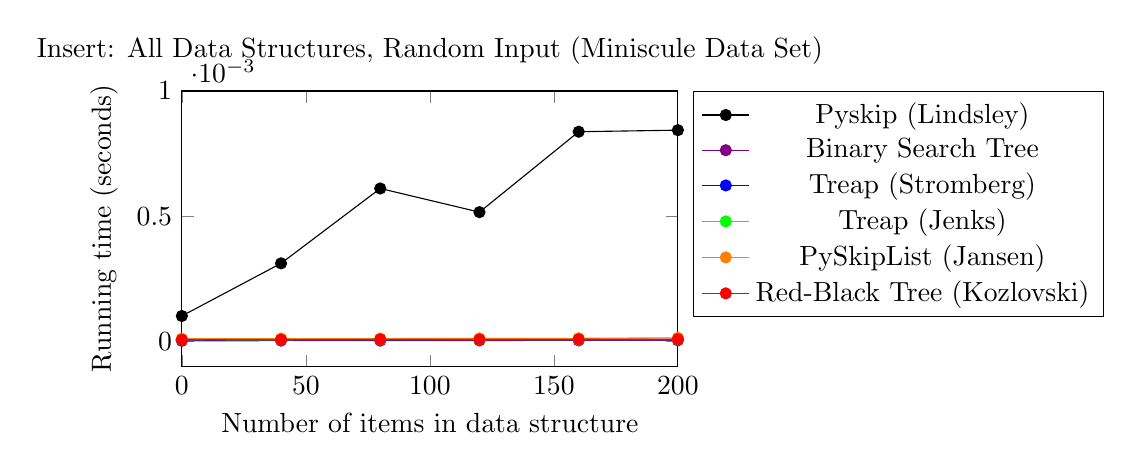
\begin{tikzpicture}
        \begin{axis}[
            title={Insert: All Data Structures, Random Input (Miniscule Data Set)},
            xmin=0, xmax=200,
            ymin=-0.0001, ymax=0.0010,
            xlabel={Number of items in data structure},
            ylabel={Running time (seconds)},
            width=0.65\textwidth,
            height=2in,
            legend pos=outer north east,
        ]
		% Pyskip
		\addplot[
		    color=black, 
		    mark=*,
	    ]
		coordinates {
			(0, 0.00010143585341796358)
			(40, 0.000311535768335931)
			(80, 0.0006105426426629923)
			(120, 0.0005160940570576679)
			(160, 0.0008371770835686271)
			(200, 0.0008434114130393855)
		};
        % BST
		\addplot[
		    color=violet,
		    mark=*,
	    ]
		coordinates {
			(0, 2.1082273572617137e-06)
			(40, 2.8912832328160653e-06)
			(80, 2.9816358338415635e-06)
			(120, 3.6743391083704157e-06)
			(160, 3.7646917093959164e-06)
			(200, 3.794809243071076e-06)
		};
		% Stromberg treap
		\addplot[
		    color=blue,
		    mark=*,
	    ]
        coordinates {
			(0, 5.1500982584523625e-06)
			(40, 6.6559749422101525e-06)
			(80, 6.3849171391350264e-06)
			(120, 6.987267812638698e-06)
			(160, 7.318560683064468e-06)
			(200, 7.288443149391921e-06)
		};
		% Jenks treap
		\addplot[
		    color=green,
		    mark=*,
	    ]
		coordinates {
			(0, 6.776445076911442e-06)
			(40, 6.625857408537605e-06)
			(80, 7.318560683064468e-06)
			(120, 6.9270327452880535e-06)
			(160, 6.776445076911442e-06)
			(200, 7.318560683064468e-06)
		};
		% PySkipList
		\addplot[
		    color=orange,
		    mark=*,
	    ]
         coordinates {
			(0, 1.0511019252634756e-05)
			(40, 1.1294075128187587e-05)
			(80, 1.108325239246033e-05)
			(120, 1.1986778402717224e-05)
			(160, 1.2287953739470447e-05)
			(200, 1.424559342835252e-05)
		};
		% Red-black tree
		\addplot[
		    color=red, 
		    mark=*,
	    ]
         coordinates {
			(0, 6.8366801442620865e-06)
			(40, 6.776445076911442e-06)
			(80, 8.101616558620073e-06)
			(120, 7.348678216742566e-06)
			(160, 8.342556828022651e-06)
			(200, 8.463026962721166e-06)
		};
        \legend{Pyskip (Lindsley), Binary Search Tree, Treap (Stromberg), Treap (Jenks), PySkipList (Jansen), Red-Black Tree (Kozlovski)}
        \end{axis}
    \end{tikzpicture}
    \caption{Average of 10 operations, benchmarked every 40, starting at 0.}
\end{figure}

Clearly Pyskip is too slow for further consideration. In fact, I began with a 105-million-element benchmark that my reference BST implementation handled in about a minute. Pyskip took so long that I eventually had to cancel the benchmark. I had to pare the initial benchmark down to below 1,000 elements to achieve a running time that would not dwarf the rest of my benchmarks combined. With Pyskip eliminated, a graph with larger (but still quite modest) data sets presents a clearer picture of the comparability of the various data structures with random inputs:

\begin{figure}[h]
    \centering
    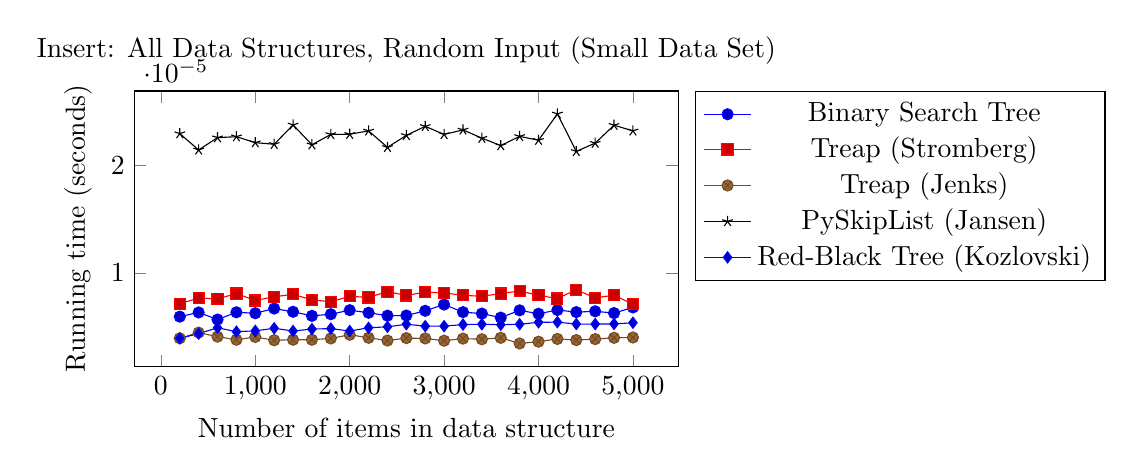
\begin{tikzpicture}
        \begin{axis}[
            xlabel={Number of items in data structure},
            ylabel={Running time (seconds)},
            title={Insert: All Data Structures, Random Input (Small Data Set)},
            width=0.7\textwidth,
            height=2in,
            legend pos=outer north east
        ]
		\addplot coordinates {
			(200, 5.933154134041274e-06)
			(400, 6.324682071845444e-06)
			(600, 5.662096330993905e-06)
			(800, 6.3397408387011465e-06)
			(1000, 6.249388237655751e-06)
			(1200, 6.686092475849392e-06)
			(1400, 6.384917139090618e-06)
			(1600, 6.00844796814215e-06)
			(1800, 6.159035636521537e-06)
			(2000, 6.535504807558823e-06)
			(2200, 6.29456453813404e-06)
			(2400, 6.023506734997852e-06)
			(2600, 6.0385655018535545e-06)
			(2800, 6.475269740136014e-06)
			(3000, 7.062561646886678e-06)
			(3200, 6.354799605468031e-06)
			(3400, 6.219270703944346e-06)
			(3600, 5.842801532995878e-06)
			(3800, 6.520446040703121e-06)
			(4000, 6.204211937088644e-06)
			(4200, 6.550563574414525e-06)
			(4400, 6.354799605468031e-06)
			(4600, 6.430093439568907e-06)
			(4800, 6.264447004422635e-06)
			(5000, 6.7915038437504904e-06)
		};
		\addplot coordinates {
			(200, 7.137855480987554e-06)
			(400, 7.664912320315409e-06)
			(600, 7.5896184861257154e-06)
			(800, 8.086557791830984e-06)
			(1000, 7.439030817746328e-06)
			(1200, 7.785382454983391e-06)
			(1400, 8.01126395764129e-06)
			(1600, 7.499265885169137e-06)
			(1800, 7.318560683078346e-06)
			(2000, 7.830558755550498e-06)
			(2200, 7.7251473876494e-06)
			(2400, 8.267262993832958e-06)
			(2600, 7.905852589740191e-06)
			(2800, 8.222086693265851e-06)
			(3000, 8.146792859164976e-06)
			(3200, 7.920911356507076e-06)
			(3400, 7.830558755550498e-06)
			(3600, 8.086557791742166e-06)
			(3800, 8.327498061166948e-06)
			(4000, 7.920911356595894e-06)
			(4200, 7.61973601983712e-06)
			(4400, 8.43290942897923e-06)
			(4600, 7.695029853937996e-06)
			(4800, 7.920911356595894e-06)
			(5000, 7.092679180509265e-06)
		};
		\addplot coordinates {
			(200, 3.915279377775249e-06)
			(400, 4.4423362171031044e-06)
			(600, 4.0658670461546365e-06)
			(800, 3.7797504762515643e-06)
			(1000, 4.035749512443232e-06)
			(1200, 3.7345741756844575e-06)
			(1400, 3.7797504761627465e-06)
			(1600, 3.7797504762515643e-06)
			(1800, 3.900220611008365e-06)
			(2000, 4.246572248156611e-06)
			(2200, 3.960455678342356e-06)
			(2400, 3.7044566420618706e-06)
			(2600, 3.930338144630951e-06)
			(2800, 3.900220610919547e-06)
			(3000, 3.6893978752061685e-06)
			(3200, 3.885161844152662e-06)
			(3400, 3.824926776729854e-06)
			(3600, 3.960455678342356e-06)
			(3800, 3.433398838925683e-06)
			(4000, 3.5990452741607727e-06)
			(4200, 3.855044310441258e-06)
			(4400, 3.7496329425401596e-06)
			(4600, 3.839985543585556e-06)
			(4800, 3.960455678253538e-06)
			(5000, 3.990573211964943e-06)
		};
		\addplot coordinates {
			(200, 2.2994736960946228e-05)
			(400, 2.147380151038547e-05)
			(600, 2.261826778999776e-05)
			(800, 2.2708620391043154e-05)
			(1000, 2.2151446018092714e-05)
			(1200, 2.2000858349713327e-05)
			(1400, 2.3807910370177156e-05)
			(1600, 2.195568204914622e-05)
			(1800, 2.2919443126845353e-05)
			(2000, 2.2934501893612236e-05)
			(2200, 2.3250735997226712e-05)
			(2400, 2.1714741779810254e-05)
			(2600, 2.2829090525799955e-05)
			(2800, 2.367238146865347e-05)
			(3000, 2.2919443126845353e-05)
			(3200, 2.334108859827211e-05)
			(3400, 2.257309148951947e-05)
			(3600, 2.1880388215045343e-05)
			(3800, 2.273873792475456e-05)
			(4000, 2.2377327520661795e-05)
			(4200, 2.483190651512146e-05)
			(4400, 2.1338272608861786e-05)
			(4600, 2.2106269717614425e-05)
			(4800, 2.3777792836554566e-05)
			(5000, 2.3250735997226712e-05)
		};
		\addplot coordinates {
			(200, 3.915279377775249e-06)
			(400, 4.351983616057708e-06)
			(600, 4.894099222241266e-06)
			(800, 4.5326888180596825e-06)
			(1000, 4.607982652338194e-06)
			(1200, 4.848922921762977e-06)
			(1400, 4.592923885482492e-06)
			(1600, 4.773629087484465e-06)
			(1800, 4.8188053880515724e-06)
			(2000, 4.592923885393674e-06)
			(2200, 4.894099222241266e-06)
			(2400, 4.984451823286662e-06)
			(2600, 5.225392092622627e-06)
			(2800, 5.044686890620653e-06)
			(3000, 5.044686890620653e-06)
			(3200, 5.1952745590000404e-06)
			(3400, 5.225392092622627e-06)
			(3600, 5.180215792144338e-06)
			(3800, 5.225392092711445e-06)
			(4000, 5.406097294713419e-06)
			(4200, 5.421156061480304e-06)
			(4400, 5.2404508594783294e-06)
			(4600, 5.2404508594783294e-06)
			(4800, 5.2555096263340316e-06)
			(5000, 5.360920994146312e-06)
		};
        \legend{Binary Search Tree, Treap (Stromberg), Treap (Jenks), PySkipList (Jansen), Red-Black Tree (Kozlovski)}
        \end{axis}
    \end{tikzpicture}
    \caption{Average of 20 operations, benchmarked every 200, starting at 200.}
\end{figure}

Based on these benchmark results, the only remaining skiplist implementation is again the clear outlier, but in this case, the difference is much less pronounced. Compared to the binary search tree reference implementation, PySkipList benchmarks on insertion at only about 2.5 times slower, and this, of course, is under ideal conditions for a binary search tree.

Comparing the Stromberg and Jenks treaps, the latter appears to be two or three times after in this particular benchmark. Interestingly, both are comparable or superior to the binary search tree, and the Jenks treap is even faster than the Sysoev red-black tree! Because the treaps provide such interesting counterpoints, both to one another and to the deterministic data structures used here, I will keep both. Thus, the data structures are finalized.

\section{Choosing Inputs \& Benchmarks}
- Randomized
- Well-known worst case
- Real-world data sets?

- Use a single ISDBenchmark class to produce 3 standard benchmarks
- Update the project files section to describe/list it
- Update the project files section's description of BenchmarkPlot accordingly

\todo{Finish this section}

\todo{Write something like an ISDBenchmark class that produces 3 Plots}

\todo{Section: Asymptotic Expectations - talk about expected/average performance. (Talk about it in each subjection.)}
\newpage



% \section{Candidates}
% \begin{figure}[h]
    \centering
    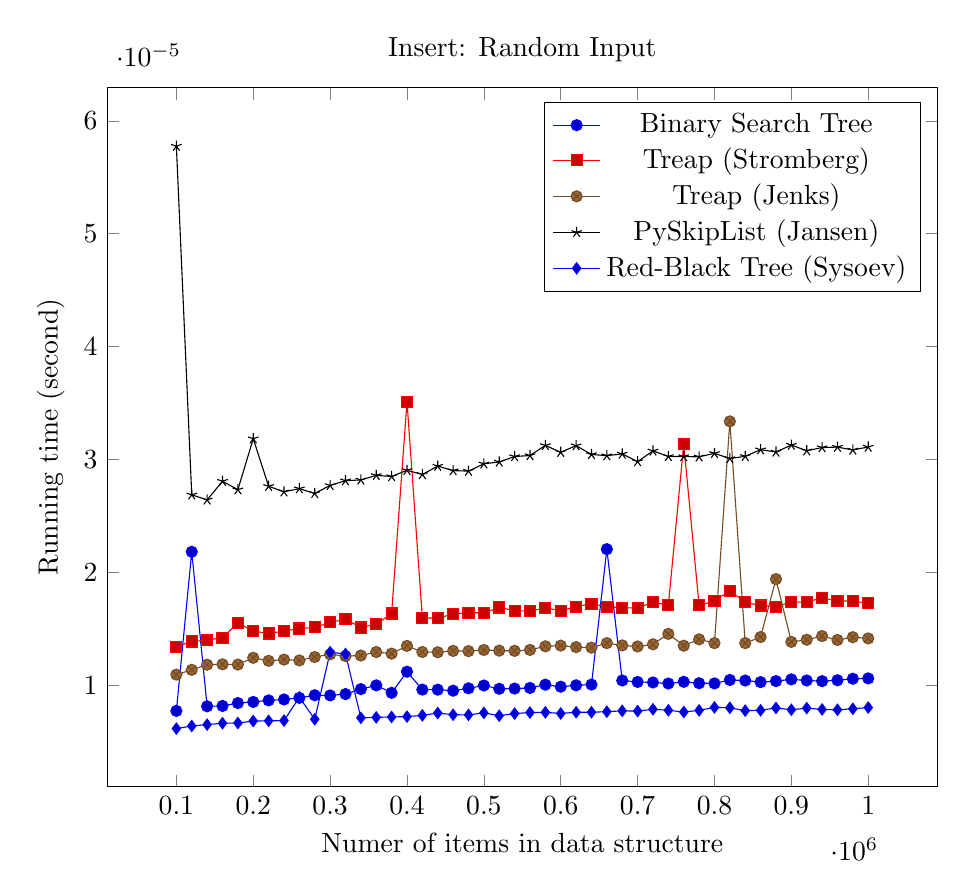
\begin{tikzpicture}
        \begin{axis}[
            xlabel={Numer of items in data structure},
            ylabel={Running time (second)},
            title={Insert: Random Input},
            width=\textwidth
        ]
		\addplot coordinates {
			(100000, 7.738700277834248e-06)
			(120000, 2.1829188407761296e-05)
			(140000, 8.143479930428466e-06)
			(160000, 8.177813918818223e-06)
			(180000, 8.434114130393856e-06)
			(200000, 8.531092588828005e-06)
			(220000, 8.672042646427735e-06)
			(240000, 8.750649409319911e-06)
			(260000, 8.89039476557274e-06)
			(280000, 9.125311528239034e-06)
			(300000, 9.109650410727977e-06)
			(320000, 9.229217019417923e-06)
			(340000, 9.665620082371263e-06)
			(360000, 1.0000225881502622e-05)
			(380000, 9.339146017332655e-06)
			(400000, 1.121064955990736e-05)
			(420000, 9.623455535226366e-06)
			(440000, 9.618335554501645e-06)
			(460000, 9.52768177813912e-06)
			(480000, 9.73850451386582e-06)
			(500000, 9.987576517358932e-06)
			(520000, 9.693328213352892e-06)
			(540000, 9.715012837598458e-06)
			(560000, 9.771633800908397e-06)
			(580000, 1.0058352721495467e-05)
			(600000, 9.880960448149345e-06)
			(620000, 1.000504468689023e-05)
			(640000, 1.0070098559629593e-05)
			(660000, 2.2063502819754e-05)
			(680000, 1.0431810139068354e-05)
			(700000, 1.030320827027431e-05)
			(720000, 1.0257429619088931e-05)
			(740000, 1.0161655862001239e-05)
			(760000, 1.0313749407060868e-05)
			(780000, 1.0189665168319095e-05)
			(800000, 1.017490757681827e-05)
			(820000, 1.0477588790253733e-05)
			(840000, 1.0426690158341856e-05)
			(860000, 1.0287848328101034e-05)
			(880000, 1.0377899753789777e-05)
			(900000, 1.0531800350868536e-05)
			(920000, 1.0432713665077031e-05)
			(940000, 1.037217742238994e-05)
			(960000, 1.0453494763313032e-05)
			(980000, 1.0587517788168909e-05)
			(1000000, 1.0616129445159217e-05)
		};
		\addplot coordinates {
			(100000, 1.3428203564410878e-05)
			(120000, 1.3885990076271781e-05)
			(140000, 1.3997424950870752e-05)
			(160000, 1.4225715856127863e-05)
			(180000, 1.5524685083539325e-05)
			(200000, 1.4806984256058087e-05)
			(220000, 1.4597667397016068e-05)
			(240000, 1.4808490132743658e-05)
			(260000, 1.5033166933957177e-05)
			(280000, 1.5136168899129387e-05)
			(300000, 1.5575583715449425e-05)
			(320000, 1.5858989707332683e-05)
			(340000, 1.5119604255609432e-05)
			(360000, 1.5408732578887196e-05)
			(380000, 1.6362554870383405e-05)
			(400000, 3.512126071996136e-05)
			(420000, 1.5975845737990825e-05)
			(440000, 1.595476346442126e-05)
			(460000, 1.631828209588093e-05)
			(480000, 1.643724635389887e-05)
			(500000, 1.6422187587057378e-05)
			(520000, 1.6897743443788473e-05)
			(540000, 1.662036095864039e-05)
			(560000, 1.6570064677402742e-05)
			(580000, 1.6853470669285995e-05)
			(600000, 1.6612530399886083e-05)
			(620000, 1.695376205642418e-05)
			(640000, 1.7230241015564473e-05)
			(660000, 1.6955569108446868e-05)
			(680000, 1.688238350161342e-05)
			(700000, 1.6839014253122285e-05)
			(720000, 1.7366974618447273e-05)
			(740000, 1.7084773327912474e-05)
			(760000, 3.1351147854500993e-05)
			(780000, 1.708146039920777e-05)
			(800000, 1.7463651901543644e-05)
			(820000, 1.8385549607344842e-05)
			(840000, 1.7348000572230405e-05)
			(860000, 1.707272631444212e-05)
			(880000, 1.6970627875284807e-05)
			(900000, 1.737781693057272e-05)
			(920000, 1.7375106352538693e-05)
			(940000, 1.7748864945449584e-05)
			(960000, 1.7464856602892098e-05)
			(980000, 1.747690361636245e-05)
			(1000000, 1.7261262075251694e-05)
		};
		\addplot coordinates {
			(100000, 1.0951337594963917e-05)
			(120000, 1.1375693644446017e-05)
			(140000, 1.1831070753615336e-05)
			(160000, 1.1864200040655248e-05)
			(180000, 1.1841611890396564e-05)
			(200000, 1.2440047284528077e-05)
			(220000, 1.2172302410156988e-05)
			(240000, 1.2280123180708813e-05)
			(260000, 1.2209045801242269e-05)
			(280000, 1.2510221137986832e-05)
			(300000, 1.2746944952674255e-05)
			(320000, 1.2594249056938621e-05)
			(340000, 1.2641533584812238e-05)
			(360000, 1.2950539480321765e-05)
			(380000, 1.281109529940494e-05)
			(400000, 1.3494462138496033e-05)
			(420000, 1.29535512336858e-05)
			(440000, 1.2932770135456906e-05)
			(460000, 1.3049626166115047e-05)
			(480000, 1.3030350944561064e-05)
			(500000, 1.3134256435741065e-05)
			(520000, 1.3075828420411994e-05)
			(540000, 1.305324027015331e-05)
			(560000, 1.3138472890460662e-05)
			(580000, 1.345741757207719e-05)
			(600000, 1.3521869094141436e-05)
			(620000, 1.338724371861133e-05)
			(640000, 1.3341163892093278e-05)
			(660000, 1.3738715336600648e-05)
			(680000, 1.3540843140354752e-05)
			(700000, 1.3443563506584154e-05)
			(720000, 1.3634809845420647e-05)
			(740000, 1.4563032233290585e-05)
			(760000, 1.3512833834042226e-05)
			(780000, 1.407693523977116e-05)
			(800000, 1.3740823563956895e-05)
			(820000, 3.337956374753048e-05)
			(840000, 1.3739920037949106e-05)
			(860000, 1.4276915663373302e-05)
			(880000, 1.9411352804318936e-05)
			(900000, 1.3850150211197843e-05)
			(920000, 1.4041697725367896e-05)
			(940000, 1.4363352985022005e-05)
			(960000, 1.4020013101131213e-05)
			(980000, 1.4265772175917845e-05)
			(1000000, 1.4157349054684687e-05)
		};
		\addplot coordinates {
			(100000, 5.7758803731559285e-05)
			(120000, 2.6875381175038625e-05)
			(140000, 2.642391934524113e-05)
			(160000, 2.8081287223386653e-05)
			(180000, 2.732955358285949e-05)
			(200000, 3.18456777574454e-05)
			(220000, 2.7632837146967405e-05)
			(240000, 2.7143728400083943e-05)
			(260000, 2.7419303833212895e-05)
			(280000, 2.6997959537091275e-05)
			(300000, 2.7705119227782405e-05)
			(320000, 2.8130077627942286e-05)
			(340000, 2.8192420922650285e-05)
			(360000, 2.8596297049240605e-05)
			(380000, 2.8497812714114446e-05)
			(400000, 2.9045048300993414e-05)
			(420000, 2.867881909150327e-05)
			(440000, 2.9417903367900067e-05)
			(460000, 2.9019448397370694e-05)
			(480000, 2.8976079148890223e-05)
			(500000, 2.9620895544866245e-05)
			(520000, 2.9785638454072227e-05)
			(540000, 3.02663142915236e-05)
			(560000, 3.0355763366529232e-05)
			(580000, 3.1248145889335886e-05)
			(600000, 3.064489168981765e-05)
			(620000, 3.123067771980459e-05)
			(640000, 3.0449127720928004e-05)
			(660000, 3.0345222229740898e-05)
			(680000, 3.0493099320096917e-05)
			(700000, 2.9820273617801264e-05)
			(720000, 3.07617477204758e-05)
			(740000, 3.0277758954312616e-05)
			(760000, 3.026420606416025e-05)
			(780000, 3.02422202645829e-05)
			(800000, 3.054911793273618e-05)
			(820000, 3.00901267195286e-05)
			(840000, 3.0284083636388458e-05)
			(860000, 3.0871977893738746e-05)
			(880000, 3.066808219074346e-05)
			(900000, 3.128368457906561e-05)
			(920000, 3.077771001332508e-05)
			(940000, 3.1059911303870536e-05)
			(960000, 3.110237702634322e-05)
			(980000, 3.084788386679804e-05)
			(1000000, 3.110840053307129e-05)
		};
		\addplot coordinates {
			(100000, 6.17198617604231e-06)
			(120000, 6.403288834675891e-06)
			(140000, 6.522253092697383e-06)
			(160000, 6.6442291040829105e-06)
			(180000, 6.662299624281332e-06)
			(200000, 6.839691897639e-06)
			(220000, 6.855654190488281e-06)
			(240000, 6.881856444778123e-06)
			(260000, 8.939787520802156e-06)
			(280000, 6.996001897405791e-06)
			(300000, 1.2935480713480273e-05)
			(320000, 1.277676131101657e-05)
			(340000, 7.12249553883737e-06)
			(360000, 7.164961261324265e-06)
			(380000, 7.200499951053985e-06)
			(400000, 7.233328062767441e-06)
			(420000, 7.3423535346677224e-06)
			(440000, 7.548056289678584e-06)
			(460000, 7.39716744595853e-06)
			(480000, 7.383915731139723e-06)
			(500000, 7.564018582513654e-06)
			(520000, 7.313139526999634e-06)
			(540000, 7.4986635344345135e-06)
			(560000, 7.593232590181742e-06)
			(580000, 7.608893707697462e-06)
			(600000, 7.511312898586198e-06)
			(620000, 7.617326617122444e-06)
			(640000, 7.617627792456005e-06)
			(660000, 7.668225249034321e-06)
			(680000, 7.74110968052355e-06)
			(700000, 7.722135634310234e-06)
			(720000, 7.882360913455955e-06)
			(740000, 7.792911838450323e-06)
			(760000, 7.640517118048252e-06)
			(780000, 7.785081279692464e-06)
			(800000, 8.051019102040868e-06)
			(820000, 8.011263957584446e-06)
			(840000, 7.764300181449358e-06)
			(860000, 7.79230948776899e-06)
			(880000, 8.000421645476763e-06)
			(900000, 7.839594015649708e-06)
			(920000, 7.982652300597693e-06)
			(940000, 7.866699795954446e-06)
			(960000, 7.832365807558971e-06)
			(980000, 7.925730161957744e-06)
			(1000000, 8.03535798453936e-06)
		};
        \legend{Binary Search Tree, Treap (Stromberg), Treap (Jenks), PySkipList (Jansen), Red-Black Tree (Sysoev)}
        \end{axis}
    \end{tikzpicture}
    \caption{Average of 1000 operations, benchmarked every 20000, starting at 100000.}
\end{figure}
% \begin{figure}[h]
    \centering
    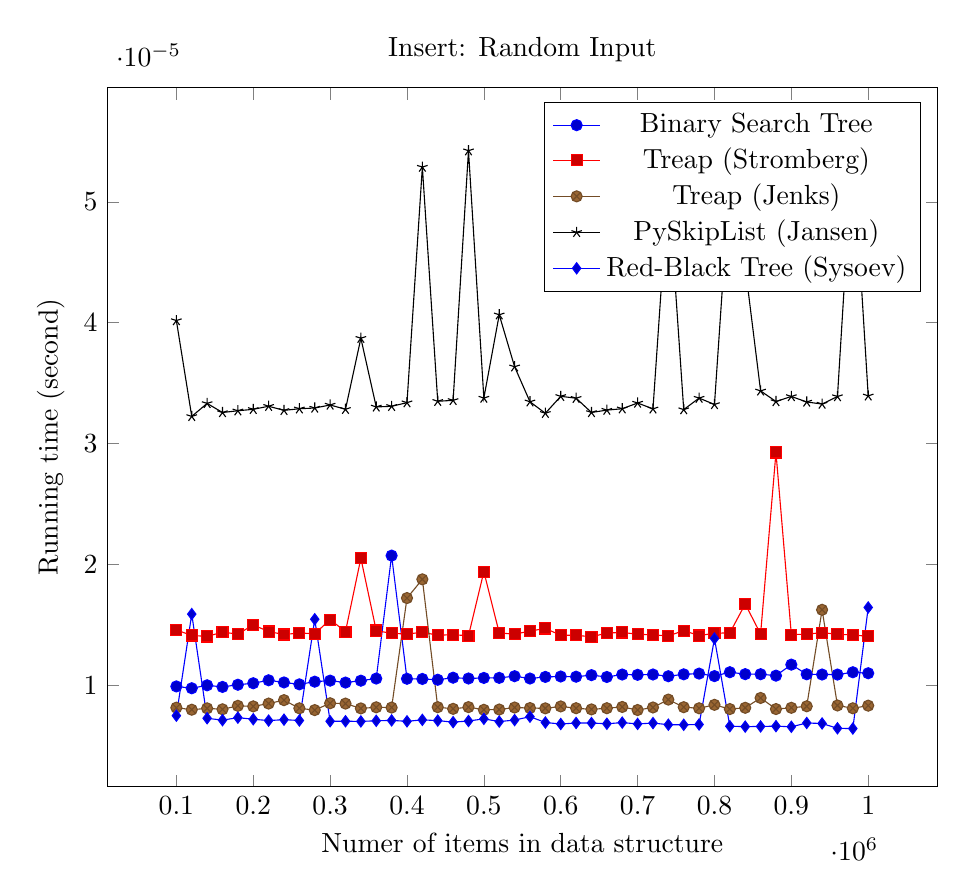
\begin{tikzpicture}
        \begin{axis}[
            xlabel={Numer of items in data structure},
            ylabel={Running time (second)},
            title={Insert: Random Input},
            width=\textwidth
        ]
		\addplot coordinates {
			(100000, 9.890899234264339e-06)
			(120000, 9.737299812513812e-06)
			(140000, 9.98215536129976e-06)
			(160000, 9.84783116109611e-06)
			(180000, 1.0028235187832023e-05)
			(200000, 1.0152319426566691e-05)
			(220000, 1.0398379676686886e-05)
			(240000, 1.0219481526647201e-05)
			(260000, 1.0060762124183498e-05)
			(280000, 1.0282125996710079e-05)
			(300000, 1.0368864493685237e-05)
			(320000, 1.0207133337843288e-05)
			(340000, 1.0365250389639869e-05)
			(360000, 1.0540835610981958e-05)
			(380000, 2.0716947889127368e-05)
			(400000, 1.0522463915435764e-05)
			(420000, 1.0506802797920045e-05)
			(440000, 1.0441447749840904e-05)
			(460000, 1.0612214165789169e-05)
			(480000, 1.0546557942376467e-05)
			(500000, 1.0592637768894519e-05)
			(520000, 1.0597155398940573e-05)
			(540000, 1.0736599579857397e-05)
			(560000, 1.0542040312330414e-05)
			(580000, 1.0676665687853415e-05)
			(600000, 1.071130085156824e-05)
			(620000, 1.0692929156036257e-05)
			(640000, 1.0823639252180329e-05)
			(660000, 1.0670943356444696e-05)
			(680000, 1.087363435807731e-05)
			(700000, 1.0848937980469486e-05)
			(720000, 1.0876646111455557e-05)
			(740000, 1.0733587826493363e-05)
			(760000, 1.0891102527608609e-05)
			(780000, 1.095043406895968e-05)
			(800000, 1.0743526612614574e-05)
			(820000, 1.1065784222935803e-05)
			(840000, 1.090495659309454e-05)
			(860000, 1.090104131371561e-05)
			(880000, 1.0781474705041205e-05)
			(900000, 1.1694337150728983e-05)
			(920000, 1.0893813105653294e-05)
			(940000, 1.0874537884092206e-05)
			(960000, 1.086941790336482e-05)
			(980000, 1.1062170118890436e-05)
			(1000000, 1.0980551602628452e-05)
		};
		\addplot coordinates {
			(100000, 1.4560924005934339e-05)
			(120000, 1.4108859825469722e-05)
			(140000, 1.4028747185889756e-05)
			(160000, 1.4380218803879074e-05)
			(180000, 1.4223306453430951e-05)
			(200000, 1.49801600746855e-05)
			(220000, 1.4431719786472285e-05)
			(240000, 1.4186563062352775e-05)
			(260000, 1.4309743775072547e-05)
			(280000, 1.425101458441702e-05)
			(300000, 1.5418671364997748e-05)
			(320000, 1.44265998057449e-05)
			(340000, 2.0497391068644787e-05)
			(360000, 1.451153125070448e-05)
			(380000, 1.427842154005532e-05)
			(400000, 1.4230534661507477e-05)
			(420000, 1.4366063563045372e-05)
			(440000, 1.413415855375888e-05)
			(460000, 1.4166986665458125e-05)
			(480000, 1.4085669324543914e-05)
			(500000, 1.9386355251370446e-05)
			(520000, 1.4319080210526636e-05)
			(540000, 1.42112594399606e-05)
			(560000, 1.4473583158263637e-05)
			(580000, 1.468561059535034e-05)
			(600000, 1.4126026819667458e-05)
			(620000, 1.4123316241636985e-05)
			(640000, 1.399381084682716e-05)
			(660000, 1.4312454353103021e-05)
			(680000, 1.4355221250923479e-05)
			(700000, 1.4210958264627038e-05)
			(720000, 1.415403612598709e-05)
			(740000, 1.407301996039223e-05)
			(760000, 1.4509423023341128e-05)
			(780000, 1.4098318688681389e-05)
			(800000, 1.4288059150828757e-05)
			(820000, 1.432600724325539e-05)
			(840000, 1.6710713559660917e-05)
			(860000, 1.4227522908143441e-05)
			(880000, 2.9254967510709662e-05)
			(900000, 1.4176925451579336e-05)
			(920000, 1.4216078245354424e-05)
			(940000, 1.4341969536118882e-05)
			(960000, 1.4205235933218319e-05)
			(980000, 1.4151024372608844e-05)
			(1000000, 1.4035071867965599e-05)
		};
		\addplot coordinates {
			(100000, 8.130529390953712e-06)
			(120000, 7.961268851687465e-06)
			(140000, 8.073908427647326e-06)
			(160000, 7.996205190750061e-06)
			(180000, 8.282924111341572e-06)
			(200000, 8.23714546015708e-06)
			(220000, 8.469351644791346e-06)
			(240000, 8.754263513367278e-06)
			(260000, 8.07692018101136e-06)
			(280000, 7.929946616670236e-06)
			(300000, 8.497662126444539e-06)
			(320000, 8.467243417427994e-06)
			(340000, 8.069993148254184e-06)
			(360000, 8.161249275289606e-06)
			(380000, 8.138962300378694e-06)
			(400000, 1.7204038761263974e-05)
			(420000, 1.8753585868850563e-05)
			(440000, 8.172995113426396e-06)
			(460000, 8.032948581842448e-06)
			(480000, 8.176609217471764e-06)
			(500000, 7.953438292943815e-06)
			(520000, 7.977532319870305e-06)
			(540000, 8.143479930424747e-06)
			(560000, 8.099809506589395e-06)
			(580000, 8.074510778314448e-06)
			(600000, 8.234736057460168e-06)
			(620000, 8.085955441117676e-06)
			(640000, 7.98807345665864e-06)
			(660000, 8.085955441117676e-06)
			(680000, 8.189258581609237e-06)
			(700000, 7.935066597411833e-06)
			(720000, 8.147094034484326e-06)
			(740000, 8.799138638522664e-06)
			(760000, 8.16998336006236e-06)
			(780000, 8.080233109694746e-06)
			(800000, 8.366048504285572e-06)
			(820000, 8.014576886296254e-06)
			(840000, 8.120289429513151e-06)
			(860000, 8.934968715408331e-06)
			(880000, 8.015781587658921e-06)
			(900000, 8.119084728150483e-06)
			(920000, 8.245578369582063e-06)
			(940000, 1.6230338897571527e-05)
			(960000, 8.312740469676783e-06)
			(980000, 8.080233109723167e-06)
			(1000000, 8.296778176827502e-06)
		};
		\addplot coordinates {
			(100000, 4.0175886396667695e-05)
			(120000, 3.224112097458942e-05)
			(140000, 3.33154134007998e-05)
			(160000, 3.2564282110939754e-05)
			(180000, 3.2706738045220616e-05)
			(200000, 3.282811170592481e-05)
			(220000, 3.3081400164121536e-05)
			(240000, 3.27425779102839e-05)
			(260000, 3.2872986831108616e-05)
			(280000, 3.293563130114308e-05)
			(300000, 3.318590800597576e-05)
			(320000, 3.2831123459288844e-05)
			(340000, 3.871036720801158e-05)
			(360000, 3.302598390217781e-05)
			(380000, 3.307718370945167e-05)
			(400000, 3.3377455520167135e-05)
			(420000, 5.287795622416525e-05)
			(440000, 3.3493106849476816e-05)
			(460000, 3.356960538502563e-05)
			(480000, 5.423475111624043e-05)
			(500000, 3.3759948197825907e-05)
			(520000, 4.0655056357422834e-05)
			(540000, 3.6350056093908736e-05)
			(560000, 3.3451243477657044e-05)
			(580000, 3.250103529020976e-05)
			(600000, 3.3903608833469436e-05)
			(620000, 3.3745491781672855e-05)
			(640000, 3.256759503963736e-05)
			(660000, 3.276094960585851e-05)
			(680000, 3.287599858447265e-05)
			(700000, 3.334944621383329e-05)
			(720000, 3.2866059798379864e-05)
			(740000, 5.144195221851078e-05)
			(760000, 3.280462002967966e-05)
			(780000, 3.375663526912831e-05)
			(800000, 3.322927725449176e-05)
			(820000, 5.198527252605345e-05)
			(840000, 4.4608283827642484e-05)
			(860000, 3.4352058909888685e-05)
			(880000, 3.34741328032635e-05)
			(900000, 3.389156182001329e-05)
			(920000, 3.3434980009502625e-05)
			(940000, 3.3263310067525254e-05)
			(960000, 3.388493596258968e-05)
			(980000, 5.461453321586873e-05)
			(1000000, 3.3941556925924485e-05)
		};
		\addplot coordinates {
			(100000, 7.4718589294491265e-06)
			(120000, 1.5876457876856874e-05)
			(140000, 7.252000933618774e-06)
			(160000, 7.096293284547528e-06)
			(180000, 7.305007792922425e-06)
			(200000, 7.173092995401475e-06)
			(220000, 7.060453419484247e-06)
			(240000, 7.139361357701546e-06)
			(260000, 7.067982802880124e-06)
			(280000, 1.544878889868073e-05)
			(300000, 7.006844209513474e-06)
			(320000, 7.008350086238124e-06)
			(340000, 6.99389367005665e-06)
			(360000, 7.043888775939422e-06)
			(380000, 7.077319238334212e-06)
			(400000, 7.0005195274518425e-06)
			(420000, 7.120688486821792e-06)
			(440000, 7.059549893455142e-06)
			(460000, 6.931550375327333e-06)
			(480000, 7.027324132423019e-06)
			(500000, 7.204716405766476e-06)
			(520000, 6.978834903208053e-06)
			(540000, 7.103521492638265e-06)
			(560000, 7.382711029805478e-06)
			(580000, 6.904143419689035e-06)
			(600000, 6.777348602923894e-06)
			(620000, 6.864087099899053e-06)
			(640000, 6.860171820534333e-06)
			(660000, 6.798732051834122e-06)
			(680000, 6.894806984234947e-06)
			(700000, 6.7845768109862095e-06)
			(720000, 6.854750664444964e-06)
			(740000, 6.722534691647297e-06)
			(760000, 6.7113912041634194e-06)
			(780000, 6.73940051046884e-06)
			(800000, 1.3853764315229001e-05)
			(820000, 6.595438699520173e-06)
			(840000, 6.56110471115312e-06)
			(860000, 6.574657601305489e-06)
			(880000, 6.599655154246875e-06)
			(900000, 6.54755182097233e-06)
			(920000, 6.86167769720214e-06)
			(940000, 6.821019026773456e-06)
			(960000, 6.420455828873628e-06)
			(980000, 6.3999759059640835e-06)
			(1000000, 1.6424898165098513e-05)
		};
        \legend{Binary Search Tree, Treap (Stromberg), Treap (Jenks), PySkipList (Jansen), Red-Black Tree (Sysoev)}
        \end{axis}
    \end{tikzpicture}
    \caption{Average of 1000 operations, benchmarked every 20000, starting at 100000.}
\end{figure}
% \begin{figure}[h]
    \centering
    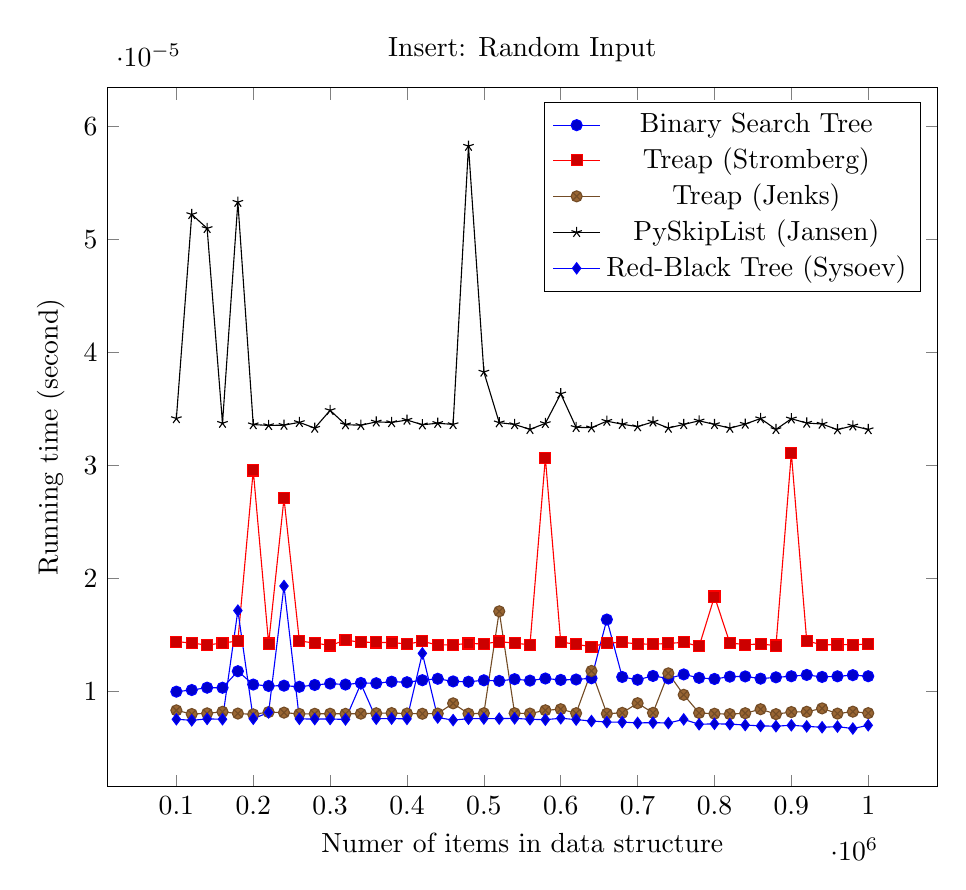
\begin{tikzpicture}
        \begin{axis}[
            xlabel={Numer of items in data structure},
            ylabel={Running time (second)},
            title={Insert: Random Input},
            width=\textwidth
        ]
		\addplot coordinates {
			(100000, 9.994804725465656e-06)
			(120000, 1.0139368887081447e-05)
			(140000, 1.0346878694093675e-05)
			(160000, 1.0339048135364237e-05)
			(180000, 1.1801254395294336e-05)
			(200000, 1.0623658828563976e-05)
			(220000, 1.0500478115858414e-05)
			(240000, 1.052366861677001e-05)
			(260000, 1.042669015834008e-05)
			(280000, 1.0586011911470904e-05)
			(300000, 1.070708439686996e-05)
			(320000, 1.0621249425867063e-05)
			(340000, 1.0764307710843468e-05)
			(360000, 1.0737503105872293e-05)
			(380000, 1.0876043760788434e-05)
			(400000, 1.0827855706878609e-05)
			(420000, 1.1008259733614523e-05)
			(440000, 1.1132946323016313e-05)
			(460000, 1.0901643664396943e-05)
			(480000, 1.0872429656728854e-05)
			(500000, 1.0998622122826874e-05)
			(520000, 1.09444105622174e-05)
			(540000, 1.109861233464926e-05)
			(560000, 1.0972419868551242e-05)
			(580000, 1.1157040349985436e-05)
			(600000, 1.1034160812556593e-05)
			(620000, 1.1069699502314733e-05)
			(640000, 1.1182037902926822e-05)
			(660000, 1.6370686604460615e-05)
			(680000, 1.1293472777509806e-05)
			(700000, 1.10474125273754e-05)
			(720000, 1.1384126553878105e-05)
			(740000, 1.1163365032018647e-05)
			(760000, 1.1520257806097333e-05)
			(780000, 1.121336013792984e-05)
			(800000, 1.1118188731529698e-05)
			(820000, 1.1321482083843648e-05)
			(840000, 1.1341660831391209e-05)
			(860000, 1.1144089810471768e-05)
			(880000, 1.1262150542478367e-05)
			(900000, 1.1355514896905561e-05)
			(920000, 1.1472973278216614e-05)
			(940000, 1.129618335554028e-05)
			(960000, 1.1350997266816876e-05)
			(980000, 1.1453698056669736e-05)
			(1000000, 1.1360032526937403e-05)
		};
		\addplot coordinates {
			(100000, 1.4419371597682584e-05)
			(120000, 1.429227560555546e-05)
			(140000, 1.4115184507545564e-05)
			(160000, 1.4302515567010231e-05)
			(180000, 1.4466656125534882e-05)
			(200000, 2.9553432269437963e-05)
			(220000, 1.4250111058402127e-05)
			(240000, 2.7089818014815137e-05)
			(260000, 1.4477197262323216e-05)
			(280000, 1.4291974430221898e-05)
			(300000, 1.4080248168482967e-05)
			(320000, 1.4547973466449094e-05)
			(340000, 1.4370280017772075e-05)
			(360000, 1.43476918675276e-05)
			(380000, 1.434166836077111e-05)
			(400000, 1.4207645335943652e-05)
			(420000, 1.4439249169896584e-05)
			(440000, 1.4123015066303425e-05)
			(460000, 1.414409733988009e-05)
			(480000, 1.4251616935069933e-05)
			(500000, 1.4218788823399109e-05)
			(520000, 1.4426298630411338e-05)
			(540000, 1.4277819189373986e-05)
			(560000, 1.4142892638545846e-05)
			(580000, 3.067169629477462e-05)
			(600000, 1.4388651713289846e-05)
			(620000, 1.4180539555610494e-05)
			(640000, 1.3968512118538002e-05)
			(660000, 1.4289565027524987e-05)
			(680000, 1.4351004796225197e-05)
			(700000, 1.4219692349399793e-05)
			(720000, 1.4186864237700546e-05)
			(740000, 1.425643574049218e-05)
			(760000, 1.435943770565018e-05)
			(780000, 1.3996521424871845e-05)
			(800000, 1.840693305624086e-05)
			(820000, 1.4297696761616408e-05)
			(840000, 1.4154036126001301e-05)
			(860000, 1.4208548861944336e-05)
			(880000, 1.4068502330360388e-05)
			(900000, 3.108490885679771e-05)
			(920000, 1.4485027821052654e-05)
			(940000, 1.4132953852424635e-05)
			(960000, 1.4157349054698897e-05)
			(980000, 1.4155240827335547e-05)
			(1000000, 1.4185057185670757e-05)
		};
		\addplot coordinates {
			(100000, 8.341954477373292e-06)
			(120000, 8.014878061658237e-06)
			(140000, 8.076016654996466e-06)
			(160000, 8.214858485246168e-06)
			(180000, 8.058849660812939e-06)
			(200000, 7.98626640462885e-06)
			(220000, 8.188355055580132e-06)
			(240000, 8.140468177060711e-06)
			(260000, 8.024816847751026e-06)
			(280000, 8.03746621187429e-06)
			(300000, 8.042586192630097e-06)
			(320000, 8.034755633843816e-06)
			(340000, 8.048910874691728e-06)
			(360000, 8.084148389087887e-06)
			(380000, 8.101014207966273e-06)
			(400000, 8.06125906348143e-06)
			(420000, 8.040779140600307e-06)
			(440000, 8.058247310117394e-06)
			(460000, 8.959966268349717e-06)
			(480000, 8.0392732639325e-06)
			(500000, 8.084148389087887e-06)
			(520000, 1.7097723867379956e-05)
			(540000, 8.087461317785483e-06)
			(560000, 8.05704260878315e-06)
			(580000, 8.347375633434239e-06)
			(600000, 8.441643513833696e-06)
			(620000, 8.087762493147466e-06)
			(640000, 1.1824444896205932e-05)
			(660000, 8.050416751387956e-06)
			(680000, 8.118783552816921e-06)
			(700000, 8.974422684531191e-06)
			(720000, 8.119084728150483e-06)
			(740000, 1.1613622160496106e-05)
			(760000, 9.716518714299127e-06)
			(780000, 8.112458870726869e-06)
			(800000, 8.042887367935237e-06)
			(820000, 8.007649853539079e-06)
			(840000, 8.08716014245192e-06)
			(860000, 8.441342338471713e-06)
			(880000, 8.007047502900378e-06)
			(900000, 8.190764458305466e-06)
			(920000, 8.216063186580414e-06)
			(940000, 8.514527945322925e-06)
			(960000, 8.054633206086238e-06)
			(980000, 8.224797271338958e-06)
			(1000000, 8.096797753211148e-06)
		};
		\addplot coordinates {
			(100000, 3.415207848627233e-05)
			(120000, 5.219579408642971e-05)
			(140000, 5.096428813445186e-05)
			(160000, 3.37358541708852e-05)
			(180000, 5.328213352606781e-05)
			(200000, 3.361267345817964e-05)
			(220000, 3.353707844865994e-05)
			(240000, 3.3560268949571534e-05)
			(260000, 3.380723272570663e-05)
			(280000, 3.330186051061901e-05)
			(300000, 3.4871285190462234e-05)
			(320000, 3.360634877608959e-05)
			(340000, 3.354942663744964e-05)
			(360000, 3.385180667555687e-05)
			(380000, 3.37991009916152e-05)
			(400000, 3.4012935480717486e-05)
			(420000, 3.359881939269371e-05)
			(440000, 3.373043301485268e-05)
			(460000, 3.362411812096866e-05)
			(480000, 5.8235564289617516e-05)
			(500000, 3.8263724183622116e-05)
			(520000, 3.3782235172765243e-05)
			(540000, 3.362200989360531e-05)
			(560000, 3.3189823285368905e-05)
			(580000, 3.371898835206366e-05)
			(600000, 3.6336503203756366e-05)
			(620000, 3.336872143540859e-05)
			(640000, 3.3335290973013796e-05)
			(660000, 3.3915655846954e-05)
			(680000, 3.364339334251554e-05)
			(700000, 3.3428052976745446e-05)
			(720000, 3.3846385519467506e-05)
			(740000, 3.330758284204194e-05)
			(760000, 3.362411812096866e-05)
			(780000, 3.394667690662345e-05)
			(800000, 3.3625021646969344e-05)
			(820000, 3.329794523125429e-05)
			(840000, 3.365845210930729e-05)
			(860000, 3.414756085624049e-05)
			(880000, 3.3181992726611046e-05)
			(900000, 3.412497270596759e-05)
			(920000, 3.374910588570401e-05)
			(940000, 3.365935563539324e-05)
			(960000, 3.3160308102367256e-05)
			(980000, 3.35015397589018e-05)
			(1000000, 3.3174463343186746e-05)
		};
		\addplot coordinates {
			(100000, 7.554380971726004e-06)
			(120000, 7.460414266688531e-06)
			(140000, 7.583896154756076e-06)
			(160000, 7.557091549756478e-06)
			(180000, 1.716338009083529e-05)
			(200000, 7.5974490449084444e-06)
			(220000, 8.154924593213764e-06)
			(240000, 1.9336661320778605e-05)
			(260000, 7.590220836846129e-06)
			(280000, 7.569138563212618e-06)
			(300000, 7.577270297360883e-06)
			(320000, 7.538719854210285e-06)
			(340000, 1.0694435032689854e-05)
			(360000, 7.601665499635146e-06)
			(380000, 7.615820740454638e-06)
			(400000, 7.587209083396829e-06)
			(420000, 1.3382424913231716e-05)
			(440000, 7.70406511406918e-06)
			(460000, 7.479990663568969e-06)
			(480000, 7.602267850302269e-06)
			(500000, 7.61642309112176e-06)
			(520000, 7.610098409031707e-06)
			(540000, 7.633891260638848e-06)
			(560000, 7.55197156900067e-06)
			(580000, 7.51583052863225e-06)
			(600000, 7.642324170092251e-06)
			(620000, 7.524865788752777e-06)
			(640000, 7.396263919929425e-06)
			(660000, 7.3083207216200206e-06)
			(680000, 7.300490162890583e-06)
			(700000, 7.2288104327071775e-06)
			(720000, 7.258325615737249e-06)
			(740000, 7.219775172643494e-06)
			(760000, 7.541129256935619e-06)
			(780000, 7.1089426486992125e-06)
			(800000, 7.150203669823441e-06)
			(820000, 7.124904941520072e-06)
			(840000, 7.042684074576755e-06)
			(860000, 6.9667878897803346e-06)
			(880000, 6.9414891614769654e-06)
			(900000, 7.0225053270291935e-06)
			(920000, 6.926430394628369e-06)
			(940000, 6.843607177017929e-06)
			(960000, 6.90143284163014e-06)
			(980000, 6.73066642576714e-06)
			(1000000, 7.020698275027826e-06)
		};
        \legend{Binary Search Tree, Treap (Stromberg), Treap (Jenks), PySkipList (Jansen), Red-Black Tree (Sysoev)}
        \end{axis}
    \end{tikzpicture}
    \caption{Average of 1000 operations, benchmarked every 20000, starting at 100000.}
\end{figure}
% \begin{figure}[h]
    \centering
    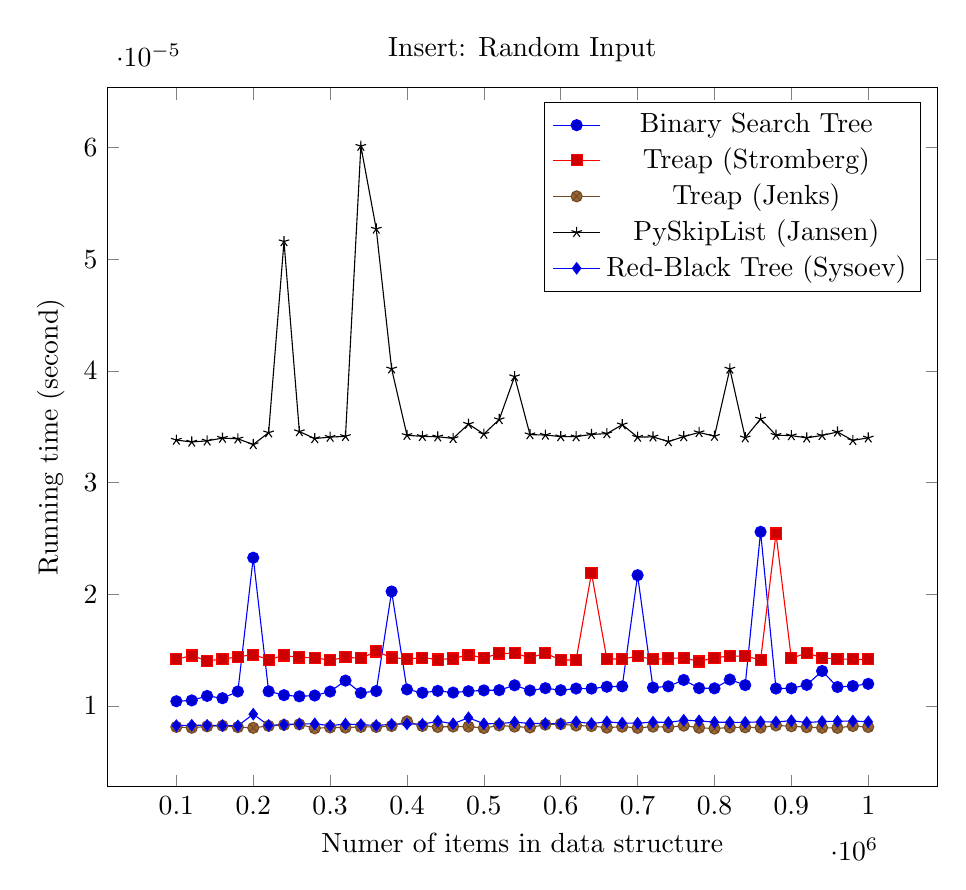
\begin{tikzpicture}
        \begin{axis}[
            xlabel={Numer of items in data structure},
            ylabel={Running time (second)},
            title={Insert: Random Input},
            width=\textwidth
        ]
		\addplot coordinates {
			(100000, 1.0411631391491483e-05)
			(120000, 1.0485720524343378e-05)
			(140000, 1.0888090774244575e-05)
			(160000, 1.0684195071291924e-05)
			(180000, 1.1285943394057085e-05)
			(200000, 2.327001121881267e-05)
			(220000, 1.1301303336267665e-05)
			(240000, 1.09561564003684e-05)
			(260000, 1.0848636805121715e-05)
			(280000, 1.0924532989974978e-05)
			(300000, 1.1277510484660525e-05)
			(320000, 1.2259342082472813e-05)
			(340000, 1.1152522719896752e-05)
			(360000, 1.1324192661845701e-05)
			(380000, 2.02441026104907e-05)
			(400000, 1.1471467401520385e-05)
			(420000, 1.1173303818168279e-05)
			(440000, 1.1340757305390525e-05)
			(460000, 1.1187459058930927e-05)
			(480000, 1.1309435070359086e-05)
			(500000, 1.1384126553878105e-05)
			(520000, 1.1404907652149632e-05)
			(540000, 1.1840708364445618e-05)
			(560000, 1.1376295995148667e-05)
			(580000, 1.158260110082665e-05)
			(600000, 1.1401293548033208e-05)
			(620000, 1.1549471813793844e-05)
			(640000, 1.154314713170379e-05)
			(660000, 1.170909474222981e-05)
			(680000, 1.174734400996158e-05)
			(700000, 2.170299594166636e-05)
			(720000, 1.163651148607414e-05)
			(740000, 1.174493460729309e-05)
			(760000, 1.2318071273170972e-05)
			(780000, 1.1585612854162263e-05)
			(800000, 1.1567241158616071e-05)
			(820000, 1.2354814664206516e-05)
			(840000, 1.1854261254541144e-05)
			(860000, 2.5588157785762178e-05)
			(880000, 1.1549772989098983e-05)
			(900000, 1.1567843509283193e-05)
			(920000, 1.1878656456815405e-05)
			(940000, 1.3119197668913785e-05)
			(960000, 1.1688915994682247e-05)
			(980000, 1.1775654491657405e-05)
			(1000000, 1.1966900830543637e-05)
		};
		\addplot coordinates {
			(100000, 1.4172106646185512e-05)
			(120000, 1.4509121847993356e-05)
			(140000, 1.403356599126937e-05)
			(160000, 1.418355130897453e-05)
			(180000, 1.4389254063985391e-05)
			(200000, 1.459074036426955e-05)
			(220000, 1.4138375008485581e-05)
			(240000, 1.4512735952052935e-05)
			(260000, 1.433203074998346e-05)
			(280000, 1.4317273158496846e-05)
			(300000, 1.4077537590480914e-05)
			(320000, 1.4352811848254986e-05)
			(340000, 1.4256736915854163e-05)
			(360000, 1.4872038128771691e-05)
			(380000, 1.4324501366559162e-05)
			(400000, 1.4196200673097792e-05)
			(420000, 1.4314863755771511e-05)
			(440000, 1.4149217320607476e-05)
			(460000, 1.4235654642277495e-05)
			(480000, 1.4573874545419585e-05)
			(500000, 1.4284143871464039e-05)
			(520000, 1.469313997881727e-05)
			(540000, 1.4713318726307989e-05)
			(560000, 1.4311852002435899e-05)
			(580000, 1.4711210498944639e-05)
			(600000, 1.411397980621132e-05)
			(620000, 1.4105245721395931e-05)
			(640000, 2.1893941105190605e-05)
			(660000, 1.4196200673154635e-05)
			(680000, 1.4203127705854968e-05)
			(700000, 1.443503271514146e-05)
			(720000, 1.4163673736732108e-05)
			(740000, 1.4247701655733636e-05)
			(760000, 1.4296492060282162e-05)
			(780000, 1.3970620345901352e-05)
			(800000, 1.4315767281857461e-05)
			(820000, 1.4455211462745865e-05)
			(840000, 1.4459126742110584e-05)
			(860000, 1.4124219767609248e-05)
			(880000, 2.543696776666593e-05)
			(900000, 1.4251315759736371e-05)
			(920000, 1.4738316279306219e-05)
			(940000, 1.4298600287645513e-05)
			(960000, 1.4196803023821757e-05)
			(980000, 1.416758901615367e-05)
			(1000000, 1.4167890191515653e-05)
		};
		\addplot coordinates {
			(100000, 8.111856520088168e-06)
			(120000, 8.035659159872921e-06)
			(140000, 8.161550450608956e-06)
			(160000, 8.216063186580414e-06)
			(180000, 8.092581298512868e-06)
			(200000, 8.029635653088007e-06)
			(220000, 8.203714997819134e-06)
			(240000, 8.289248793403203e-06)
			(260000, 8.344062704736643e-06)
			(280000, 7.988675807325762e-06)
			(300000, 8.061861414148552e-06)
			(320000, 8.049814400692412e-06)
			(340000, 8.114265922756658e-06)
			(360000, 8.108242416028588e-06)
			(380000, 8.193776211669502e-06)
			(400000, 8.610301702390188e-06)
			(420000, 8.199197367730448e-06)
			(440000, 8.107941240666605e-06)
			(460000, 8.144684631758991e-06)
			(480000, 8.143178755119606e-06)
			(500000, 8.009155730235306e-06)
			(520000, 8.242566616218028e-06)
			(540000, 8.142275229090501e-06)
			(560000, 8.063367290844781e-06)
			(580000, 8.315451047735678e-06)
			(600000, 8.363639101617081e-06)
			(620000, 8.234434882126606e-06)
			(640000, 8.185343302216098e-06)
			(660000, 8.045899121327692e-06)
			(680000, 8.132938793607991e-06)
			(700000, 8.02572037372329e-06)
			(720000, 8.134745845666202e-06)
			(740000, 8.09228012320773e-06)
			(760000, 8.223592570004711e-06)
			(780000, 8.040176789961606e-06)
			(800000, 7.96247355305013e-06)
			(820000, 8.059753186842044e-06)
			(840000, 8.076920181053992e-06)
			(860000, 8.04921205002529e-06)
			(880000, 8.245879544972468e-06)
			(900000, 8.1702845353675e-06)
			(920000, 8.087762493119045e-06)
			(940000, 8.033249757147587e-06)
			(960000, 8.0275274257815e-06)
			(980000, 8.193475036307519e-06)
			(1000000, 8.104327136607026e-06)
		};
		\addplot coordinates {
			(100000, 3.380783507640217e-05)
			(120000, 3.363797218651143e-05)
			(140000, 3.37352518202465e-05)
			(160000, 3.3985528525022346e-05)
			(180000, 3.391836642498447e-05)
			(200000, 3.341088598256192e-05)
			(220000, 3.4469216115894594e-05)
			(240000, 5.159223871157792e-05)
			(260000, 3.4569507503022124e-05)
			(280000, 3.394486985456524e-05)
			(300000, 3.4072267022054345e-05)
			(320000, 3.414424792754289e-05)
			(340000, 6.014110064529632e-05)
			(360000, 5.271893564633956e-05)
			(380000, 4.019486044290943e-05)
			(400000, 3.4235504054606736e-05)
			(420000, 3.414063382348331e-05)
			(440000, 3.4101179854360454e-05)
			(460000, 3.3957820394050484e-05)
			(480000, 3.5239321451967955e-05)
			(500000, 3.4346336578494174e-05)
			(520000, 3.565163048796194e-05)
			(540000, 3.9499145414993105e-05)
			(560000, 3.429724499864051e-05)
			(580000, 3.425869455548991e-05)
			(600000, 3.412196095263198e-05)
			(620000, 3.4112624517206315e-05)
			(640000, 3.4316219044853824e-05)
			(660000, 3.438338114494854e-05)
			(680000, 3.518510989135848e-05)
			(700000, 3.4072568197359485e-05)
			(720000, 3.409515634768923e-05)
			(740000, 3.367320970085075e-05)
			(760000, 3.4120153900630614e-05)
			(780000, 3.4488190162107915e-05)
			(800000, 3.415749964239012e-05)
			(820000, 4.0176488747363235e-05)
			(840000, 3.401715193541577e-05)
			(860000, 3.570072206787245e-05)
			(880000, 3.424785224342486e-05)
			(900000, 3.420689239760577e-05)
			(920000, 3.4004502571292506e-05)
			(940000, 3.422345704115059e-05)
			(960000, 3.4532462936624596e-05)
			(980000, 3.377591049070361e-05)
			(1000000, 3.400932137668633e-05)
		};
		\addplot coordinates {
			(100000, 8.234133706764623e-06)
			(120000, 8.263046539127571e-06)
			(140000, 8.251903051700538e-06)
			(160000, 8.23744663546222e-06)
			(180000, 8.211545556491728e-06)
			(200000, 9.25481692303265e-06)
			(220000, 8.245277194248501e-06)
			(240000, 8.316053398345958e-06)
			(260000, 8.389841355892713e-06)
			(280000, 8.387431953224223e-06)
			(300000, 8.22509844670094e-06)
			(320000, 8.368759082316046e-06)
			(340000, 8.312138119038082e-06)
			(360000, 8.242566616218028e-06)
			(380000, 8.34376152937466e-06)
			(400000, 8.383817849164644e-06)
			(420000, 8.349182685435607e-06)
			(440000, 8.624758118571662e-06)
			(460000, 8.394057810619415e-06)
			(480000, 8.937076942800104e-06)
			(500000, 8.395864862677627e-06)
			(520000, 8.405502473408432e-06)
			(540000, 8.53952549823589e-06)
			(560000, 8.420862415619013e-06)
			(580000, 8.422067116896415e-06)
			(600000, 8.394660161286539e-06)
			(620000, 8.568137155293697e-06)
			(640000, 8.413333032137872e-06)
			(660000, 8.563318349899874e-06)
			(680000, 8.46061755999017e-06)
			(700000, 8.446161143865538e-06)
			(720000, 8.545850180325942e-06)
			(740000, 8.512720893293135e-06)
			(760000, 8.709087212821487e-06)
			(780000, 8.65788740560447e-06)
			(800000, 8.53320081620268e-06)
			(820000, 8.523262030053047e-06)
			(840000, 8.518142049354083e-06)
			(860000, 8.56301717453789e-06)
			(880000, 8.553078388388258e-06)
			(900000, 8.669030893088348e-06)
			(920000, 8.502179756533224e-06)
			(940000, 8.591327656176872e-06)
			(960000, 8.616024033813119e-06)
			(980000, 8.638913359391153e-06)
			(1000000, 8.57867829205361e-06)
		};
        \legend{Binary Search Tree, Treap (Stromberg), Treap (Jenks), PySkipList (Jansen), Red-Black Tree (Sysoev)}
        \end{axis}
    \end{tikzpicture}
    \caption{Average of 1000 operations, benchmarked every 20000, starting at 100000.}
\end{figure}
% \begin{figure}[h]
    \centering
    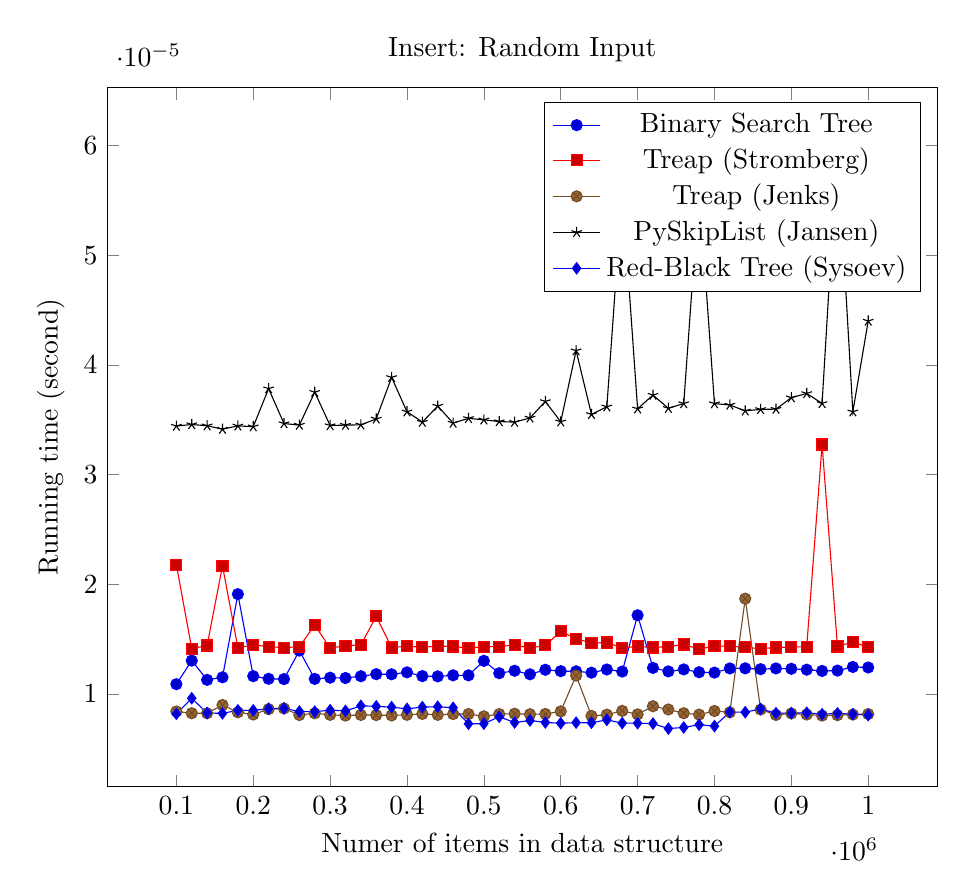
\begin{tikzpicture}
        \begin{axis}[
            xlabel={Numer of items in data structure},
            ylabel={Running time (second)},
            title={Insert: Random Input},
            width=\textwidth
        ]
		\addplot coordinates {
			(100000, 1.0878754338818907e-05)
			(120000, 1.302944741854617e-05)
			(140000, 1.1271185802627315e-05)
			(160000, 1.1505801389887438e-05)
			(180000, 1.9089998720005496e-05)
			(200000, 1.1609104530464264e-05)
			(220000, 1.1366658384361016e-05)
			(240000, 1.1340456130085386e-05)
			(260000, 1.3940803987566142e-05)
			(280000, 1.1357924299602473e-05)
			(300000, 1.1470865050853263e-05)
			(320000, 1.1441651043242018e-05)
			(340000, 1.1603683374346474e-05)
			(360000, 1.1790713258449159e-05)
			(380000, 1.1779569771022125e-05)
			(400000, 1.1956058518421742e-05)
			(420000, 1.1616031563164597e-05)
			(440000, 1.1590732834861228e-05)
			(460000, 1.1685000715317529e-05)
			(480000, 1.1685000715317529e-05)
			(500000, 1.3004449865604784e-05)
			(520000, 1.1878656456815405e-05)
			(540000, 1.2101526206038215e-05)
			(560000, 1.1777160368353634e-05)
			(580000, 1.219157763171097e-05)
			(600000, 1.206689104230918e-05)
			(620000, 1.2050025223402372e-05)
			(640000, 1.1927446861420775e-05)
			(660000, 1.2217779885986601e-05)
			(680000, 1.2028942949882548e-05)
			(700000, 1.7163380090778446e-05)
			(720000, 1.2362645222935954e-05)
			(740000, 1.204520641806539e-05)
			(760000, 1.2226513970745146e-05)
			(780000, 1.1968105531821039e-05)
			(800000, 1.1932566842119741e-05)
			(820000, 1.2314758344416532e-05)
			(840000, 1.232349242923192e-05)
			(860000, 1.2247897419683795e-05)
			(880000, 1.2315360695140498e-05)
			(900000, 1.228012318074434e-05)
			(920000, 1.2200010541107531e-05)
			(940000, 1.2084359211826267e-05)
			(960000, 1.2116584972829969e-05)
			(980000, 1.2448480193938849e-05)
			(1000000, 1.2400894490781412e-05)
		};
		\addplot coordinates {
			(100000, 2.1769254515731974e-05)
			(120000, 1.4121208014330478e-05)
			(140000, 1.44073245841696e-05)
			(160000, 2.1670167829995534e-05)
			(180000, 1.4203127705854968e-05)
			(200000, 1.4454910287383881e-05)
			(220000, 1.4298901462950652e-05)
			(240000, 1.4214572368700829e-05)
			(260000, 1.4291070904221214e-05)
			(280000, 1.6267985814636176e-05)
			(300000, 1.4160963158758477e-05)
			(320000, 1.4391964642015865e-05)
			(340000, 1.4464547898171532e-05)
			(360000, 1.7060378125620444e-05)
			(380000, 1.4216078245340214e-05)
			(400000, 1.435371537422725e-05)
			(420000, 1.4239268746280232e-05)
			(440000, 1.4350402445529653e-05)
			(460000, 1.4318779035193074e-05)
			(480000, 1.4169697243517022e-05)
			(500000, 1.4301310865675987e-05)
			(520000, 1.430070851495202e-05)
			(540000, 1.4450392657295197e-05)
			(560000, 1.4180539555638917e-05)
			(580000, 1.4418769247015462e-05)
			(600000, 1.569755972684561e-05)
			(620000, 1.5026842251870676e-05)
			(640000, 1.4628387281391042e-05)
			(660000, 1.4674165932603955e-05)
			(680000, 1.4188671289730336e-05)
			(700000, 1.4322091963890671e-05)
			(720000, 1.4229028784882303e-05)
			(740000, 1.4305226145040705e-05)
			(760000, 1.4505206568628636e-05)
			(780000, 1.4072417609725108e-05)
			(800000, 1.4360642406984426e-05)
			(820000, 1.4342571886800215e-05)
			(840000, 1.424077462297646e-05)
			(860000, 1.4114582156878441e-05)
			(880000, 1.4225715856127863e-05)
			(900000, 1.426818157864318e-05)
			(920000, 1.42925767808606e-05)
			(940000, 3.274257791025548e-05)
			(960000, 1.4317875509163968e-05)
			(980000, 1.4727473967184324e-05)
			(1000000, 1.4251014584431232e-05)
		};
		\addplot coordinates {
			(100000, 8.387431953224223e-06)
			(120000, 8.229013726065659e-06)
			(140000, 8.226604323397169e-06)
			(160000, 8.97622973656098e-06)
			(180000, 8.313041645010343e-06)
			(200000, 8.110651818697079e-06)
			(220000, 8.598857039601171e-06)
			(240000, 8.665717964333907e-06)
			(260000, 8.065776693513271e-06)
			(280000, 8.221484342641362e-06)
			(300000, 8.081136635723851e-06)
			(320000, 8.014878061601394e-06)
			(340000, 8.07300490163243e-06)
			(360000, 8.057343784116711e-06)
			(380000, 8.026322724447254e-06)
			(400000, 8.083847213754325e-06)
			(420000, 8.164863379306552e-06)
			(440000, 8.080835460361868e-06)
			(460000, 8.153117541212396e-06)
			(480000, 8.157032820577114e-06)
			(500000, 7.942595980807709e-06)
			(520000, 8.151310489211028e-06)
			(540000, 8.181126847546239e-06)
			(560000, 8.13685407297271e-06)
			(580000, 8.163658677972308e-06)
			(600000, 8.397671914678994e-06)
			(620000, 1.1662713740349773e-05)
			(640000, 7.981146423901463e-06)
			(660000, 8.096195402572447e-06)
			(680000, 8.443149390473081e-06)
			(700000, 8.12239765684808e-06)
			(720000, 8.868107790647173e-06)
			(740000, 8.569341856627943e-06)
			(760000, 8.229314901427642e-06)
			(780000, 8.10312243527278e-06)
			(800000, 8.431704727684064e-06)
			(820000, 8.30822283961652e-06)
			(840000, 1.867949673601288e-05)
			(860000, 8.562113648508785e-06)
			(880000, 8.072402550908463e-06)
			(900000, 8.20702792651673e-06)
			(920000, 8.108242416028588e-06)
			(940000, 8.012468658932904e-06)
			(960000, 8.051621452750623e-06)
			(980000, 8.111254169364201e-06)
			(1000000, 8.15432224254664e-06)
		};
		\addplot coordinates {
			(100000, 3.4424943341377914e-05)
			(120000, 3.456468869768514e-05)
			(140000, 3.4453554998378876e-05)
			(160000, 3.413942912214907e-05)
			(180000, 3.443849623153028e-05)
			(200000, 3.4367720027375984e-05)
			(220000, 3.78333446274155e-05)
			(240000, 3.465202954532742e-05)
			(260000, 3.451348889041128e-05)
			(280000, 3.751108701709427e-05)
			(300000, 3.447313139525932e-05)
			(320000, 3.450927243562774e-05)
			(340000, 3.453637821598932e-05)
			(360000, 3.5076084419415564e-05)
			(380000, 3.8863364279109194e-05)
			(400000, 3.5726321971480954e-05)
			(420000, 3.478484786876379e-05)
			(440000, 3.62488611807521e-05)
			(460000, 3.4697507021178355e-05)
			(480000, 3.512397129799183e-05)
			(500000, 3.499296002649999e-05)
			(520000, 3.483363827336916e-05)
			(540000, 3.478153494012304e-05)
			(560000, 3.516402761778181e-05)
			(580000, 3.666960312619949e-05)
			(600000, 3.48113512984014e-05)
			(620000, 4.129927040276016e-05)
			(640000, 3.548598405274106e-05)
			(660000, 3.618320495735361e-05)
			(680000, 5.5924947106063886e-05)
			(700000, 3.600069270328277e-05)
			(720000, 3.724906447411058e-05)
			(740000, 3.60461701791337e-05)
			(760000, 3.647685091067387e-05)
			(780000, 5.6013793830402394e-05)
			(800000, 3.6474140332643404e-05)
			(820000, 3.6344634937847785e-05)
			(840000, 3.5810349890425645e-05)
			(860000, 3.594226468794659e-05)
			(880000, 3.596756341619312e-05)
			(900000, 3.7011135958039174e-05)
			(920000, 3.7398447441148616e-05)
			(940000, 3.649010262546426e-05)
			(960000, 5.995888956653062e-05)
			(980000, 3.572843019884431e-05)
			(1000000, 4.400563197879137e-05)
		};
		\addplot coordinates {
			(100000, 8.171790412120572e-06)
			(120000, 9.592434475507616e-06)
			(140000, 8.25039717500431e-06)
			(160000, 8.214858485246168e-06)
			(180000, 8.49404802238496e-06)
			(200000, 8.494349197746941e-06)
			(220000, 8.6401180607254e-06)
			(240000, 8.675054399759575e-06)
			(260000, 8.385022550498888e-06)
			(280000, 8.37387906301501e-06)
			(300000, 8.506095035897942e-06)
			(320000, 8.440137637137468e-06)
			(340000, 8.903646480405314e-06)
			(360000, 8.856964303163295e-06)
			(380000, 8.78257399500626e-06)
			(400000, 8.62776987196412e-06)
			(420000, 8.784682222369611e-06)
			(440000, 8.823533840825349e-06)
			(460000, 8.72715773306254e-06)
			(480000, 7.263445596436213e-06)
			(500000, 7.274890259225231e-06)
			(520000, 7.904949063743061e-06)
			(540000, 7.382409854471916e-06)
			(560000, 7.564018582570498e-06)
			(580000, 7.387831010532864e-06)
			(600000, 7.318861858436776e-06)
			(620000, 7.369158139624687e-06)
			(640000, 7.358014652197653e-06)
			(660000, 7.623952474546059e-06)
			(680000, 7.3260900664990915e-06)
			(700000, 7.3161512803494585e-06)
			(720000, 7.285732571403969e-06)
			(740000, 6.827343708835088e-06)
			(760000, 6.932152725994456e-06)
			(780000, 7.180923554187757e-06)
			(800000, 7.053827562060633e-06)
			(820000, 8.335930970645222e-06)
			(840000, 8.31966750246238e-06)
			(860000, 8.625661644543925e-06)
			(880000, 8.2293149013708e-06)
			(900000, 8.234434882126606e-06)
			(920000, 8.271178273218993e-06)
			(940000, 8.140769352394273e-06)
			(960000, 8.212449082577678e-06)
			(980000, 8.142877579757623e-06)
			(1000000, 8.058247310145817e-06)
		};
        \legend{Binary Search Tree, Treap (Stromberg), Treap (Jenks), PySkipList (Jansen), Red-Black Tree (Sysoev)}
        \end{axis}
    \end{tikzpicture}
    \caption{Average of 1000 operations, benchmarked every 20000, starting at 100000.}
\end{figure}
% \begin{figure}[h]
    \centering
    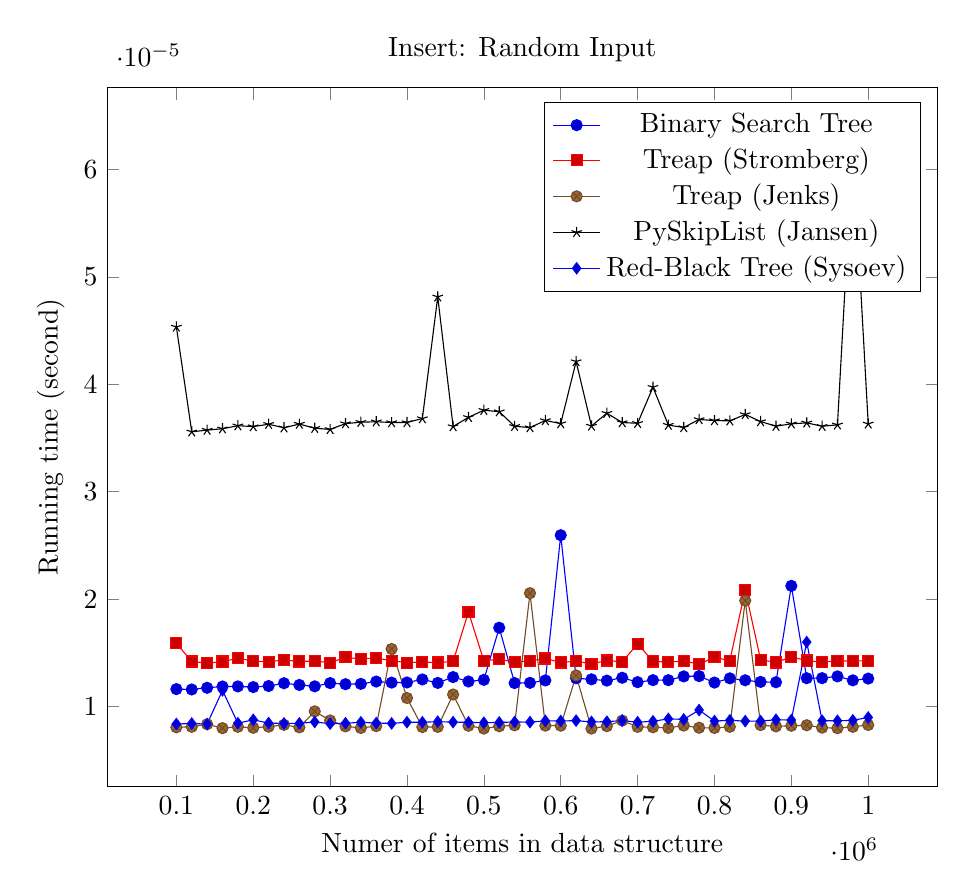
\begin{tikzpicture}
        \begin{axis}[
            xlabel={Numer of items in data structure},
            ylabel={Running time (second)},
            title={Insert: Random Input},
            width=\textwidth
        ]
		\addplot coordinates {
			(100000, 1.1623862121950879e-05)
			(120000, 1.1588323432192737e-05)
			(140000, 1.1747645185323562e-05)
			(160000, 1.1864501215995915e-05)
			(180000, 1.1876247054146915e-05)
			(200000, 1.1811494356720686e-05)
			(220000, 1.1911785743848213e-05)
			(240000, 1.2170495358134303e-05)
			(260000, 1.2010571254279512e-05)
			(280000, 1.1881668210207862e-05)
			(300000, 1.2182542371590444e-05)
			(320000, 1.2080443932404705e-05)
			(340000, 1.2110862641463883e-05)
			(360000, 1.2328010059263762e-05)
			(380000, 1.2229826899499585e-05)
			(400000, 1.2242476263622848e-05)
			(420000, 1.252317167751471e-05)
			(440000, 1.2201817593165742e-05)
			(460000, 1.2743330848593359e-05)
			(480000, 1.2334334741353814e-05)
			(500000, 1.2484320059058974e-05)
			(520000, 1.7337158260090746e-05)
			(540000, 1.2188565878318514e-05)
			(560000, 1.2206636398559567e-05)
			(580000, 1.243251790111799e-05)
			(600000, 2.5951375241902498e-05)
			(620000, 1.2635510078098378e-05)
			(640000, 1.2533712814217779e-05)
			(660000, 1.2415049731600903e-05)
			(680000, 1.2679180501891096e-05)
			(700000, 1.227048556995669e-05)
			(720000, 1.245661192803027e-05)
			(740000, 1.2456009577363148e-05)
			(760000, 1.2805071792683975e-05)
			(780000, 1.283428580029522e-05)
			(800000, 1.2230128074804725e-05)
			(820000, 1.2623764239947377e-05)
			(840000, 1.2445769615908375e-05)
			(860000, 1.2293374895534725e-05)
			(880000, 1.2263558537199514e-05)
			(900000, 2.1234065942337566e-05)
			(920000, 1.2639726532825079e-05)
			(940000, 1.2644244162856921e-05)
			(960000, 1.2808685896743555e-05)
			(980000, 1.2438240232484078e-05)
			(1000000, 1.260238079106557e-05)
		};
		\addplot coordinates {
			(100000, 1.5886396663006508e-05)
			(120000, 1.4194092445734441e-05)
			(140000, 1.4033867166631353e-05)
			(160000, 1.418776776370123e-05)
			(180000, 1.4489846626474901e-05)
			(200000, 1.4234148765524423e-05)
			(220000, 1.4172407821547495e-05)
			(240000, 1.4333235451317705e-05)
			(260000, 1.4199513601852231e-05)
			(280000, 1.4232944064190179e-05)
			(300000, 1.4087476376573704e-05)
			(320000, 1.4579898052147655e-05)
			(340000, 1.443985152059213e-05)
			(360000, 1.4516350056112514e-05)
			(380000, 1.426245924722025e-05)
			(400000, 1.4089283428575072e-05)
			(420000, 1.4142591463212284e-05)
			(440000, 1.4093198707996635e-05)
			(460000, 1.4207645335943652e-05)
			(480000, 1.8795750415961265e-05)
			(500000, 1.4260652195218881e-05)
			(520000, 1.43955787460186e-05)
			(540000, 1.4153734950639318e-05)
			(560000, 1.4239569921642215e-05)
			(580000, 1.4472980807624936e-05)
			(600000, 1.4107052773454142e-05)
			(620000, 1.421698177136932e-05)
			(640000, 1.3970921521206492e-05)
			(660000, 1.4287757975523618e-05)
			(680000, 1.4161264334063617e-05)
			(700000, 1.584362976512921e-05)
			(720000, 1.4200718303186477e-05)
			(740000, 1.415222907394309e-05)
			(760000, 1.4230835836883672e-05)
			(780000, 1.395405570241337e-05)
			(800000, 1.4583512156207234e-05)
			(820000, 1.4277819189430829e-05)
			(840000, 2.0846754459228124e-05)
			(860000, 1.4357329478286828e-05)
			(880000, 1.4104342195423669e-05)
			(900000, 1.4626279054027692e-05)
			(920000, 1.4278722715403092e-05)
			(940000, 1.4127532696363688e-05)
			(960000, 1.426276042252539e-05)
			(980000, 1.422300527809739e-05)
			(1000000, 1.427812036473597e-05)
		};
		\addplot coordinates {
			(100000, 8.069691972934834e-06)
			(120000, 8.114265922756658e-06)
			(140000, 8.35339914016231e-06)
			(160000, 7.990784034689114e-06)
			(180000, 8.11245887075529e-06)
			(200000, 8.020600393024323e-06)
			(220000, 8.12661411157478e-06)
			(240000, 8.297681702856608e-06)
			(260000, 8.06306611553964e-06)
			(280000, 9.551173454383388e-06)
			(300000, 8.708183686849224e-06)
			(320000, 8.15582811924287e-06)
			(340000, 8.007951028901062e-06)
			(360000, 8.176910392762693e-06)
			(380000, 1.5359038648284697e-05)
			(400000, 1.0793822893845118e-05)
			(420000, 8.093183649236835e-06)
			(440000, 8.105230662636131e-06)
			(460000, 1.1120598134198189e-05)
			(480000, 8.211846731853711e-06)
			(500000, 7.949221838202902e-06)
			(520000, 8.162453976638062e-06)
			(540000, 8.258528909038887e-06)
			(560000, 2.0551903804630455e-05)
			(580000, 8.222387868670467e-06)
			(600000, 8.218171413943764e-06)
			(620000, 1.2893617341717344e-05)
			(640000, 7.952835942262482e-06)
			(660000, 8.17510334081817e-06)
			(680000, 8.694329621334872e-06)
			(700000, 8.111254169364201e-06)
			(720000, 8.071197849574219e-06)
			(740000, 8.013974535572289e-06)
			(760000, 8.230218427399905e-06)
			(780000, 8.028430951753763e-06)
			(800000, 8.007951028901062e-06)
			(820000, 8.113061221422414e-06)
			(840000, 1.9864621686110694e-05)
			(860000, 8.272985325277205e-06)
			(880000, 8.15221401518329e-06)
			(900000, 8.211244381186589e-06)
			(920000, 8.259733610429976e-06)
			(940000, 8.037165036569149e-06)
			(960000, 7.98415817729392e-06)
			(980000, 8.11276004606043e-06)
			(1000000, 8.285935864705607e-06)
		};
		\addplot coordinates {
			(100000, 4.5336525791924486e-05)
			(120000, 3.557483077707957e-05)
			(140000, 3.573355017954327e-05)
			(160000, 3.585914029497417e-05)
			(180000, 3.614104041020028e-05)
			(200000, 3.6062132472011396e-05)
			(220000, 3.627777401305821e-05)
			(240000, 3.594949289606575e-05)
			(260000, 3.6294941007270154e-05)
			(280000, 3.590793069952269e-05)
			(300000, 3.579770052630238e-05)
			(320000, 3.633951495714882e-05)
			(340000, 3.646480389721774e-05)
			(360000, 3.651479900315735e-05)
			(380000, 3.643769811685616e-05)
			(400000, 3.644402279894621e-05)
			(420000, 3.680904730720158e-05)
			(440000, 4.813896230029968e-05)
			(460000, 3.606785480337749e-05)
			(480000, 3.6921084532423265e-05)
			(500000, 3.7585176149946165e-05)
			(520000, 3.744753902094544e-05)
			(540000, 3.608773237567675e-05)
			(560000, 3.596967164367015e-05)
			(580000, 3.6630751507800596e-05)
			(600000, 3.6338611431119714e-05)
			(620000, 4.211726261746662e-05)
			(640000, 3.611513933117294e-05)
			(660000, 3.730839601541902e-05)
			(680000, 3.643769811685616e-05)
			(700000, 3.6367223088063836e-05)
			(720000, 3.972593044363748e-05)
			(740000, 3.619705902281112e-05)
			(760000, 3.5976598676370484e-05)
			(780000, 3.672321233614184e-05)
			(800000, 3.662051154628898e-05)
			(820000, 3.659822457143491e-05)
			(840000, 3.718943175738332e-05)
			(860000, 3.6531363646645334e-05)
			(880000, 3.609827351237982e-05)
			(900000, 3.631542093012286e-05)
			(920000, 3.6406677057129854e-05)
			(940000, 3.6091045304374344e-05)
			(960000, 3.622296010178161e-05)
			(980000, 6.216831183701288e-05)
			(1000000, 3.631150565081498e-05)
		};
		\addplot coordinates {
			(100000, 8.374782589044117e-06)
			(120000, 8.42357299370633e-06)
			(140000, 8.369662608288308e-06)
			(160000, 1.1508813143336738e-05)
			(180000, 8.450979949316206e-06)
			(200000, 8.765105825546016e-06)
			(220000, 8.460918735408995e-06)
			(240000, 8.426885922290239e-06)
			(260000, 8.433511779799119e-06)
			(280000, 8.56602892781666e-06)
			(300000, 8.406104824075556e-06)
			(320000, 8.447968195923749e-06)
			(340000, 8.532899640840696e-06)
			(360000, 8.461219910600449e-06)
			(380000, 8.432307078351186e-06)
			(400000, 8.542838427047172e-06)
			(420000, 8.536212569538294e-06)
			(440000, 8.592833532929944e-06)
			(460000, 8.549464284442366e-06)
			(480000, 8.53199611481159e-06)
			(500000, 8.495252723719204e-06)
			(520000, 8.521454977994836e-06)
			(540000, 8.56361952514817e-06)
			(560000, 8.548259582994433e-06)
			(580000, 8.665115613666785e-06)
			(600000, 8.656080353603101e-06)
			(620000, 8.688607289968786e-06)
			(640000, 8.569643031933082e-06)
			(660000, 8.588315902784415e-06)
			(680000, 8.696437848698224e-06)
			(700000, 8.540730199570134e-06)
			(720000, 8.629576923908643e-06)
			(740000, 8.854554900494805e-06)
			(760000, 8.8033550931641e-06)
			(780000, 9.674052991840654e-06)
			(800000, 8.647647444149697e-06)
			(820000, 8.722640102973856e-06)
			(840000, 8.640720411335679e-06)
			(860000, 8.645539216786347e-06)
			(880000, 8.770828156912102e-06)
			(900000, 8.742216499854294e-06)
			(920000, 1.6001144466258666e-05)
			(940000, 8.67836732845717e-06)
			(960000, 8.671440295756838e-06)
			(980000, 8.718122472942014e-06)
			(1000000, 8.985264996681507e-06)
		};
        \legend{Binary Search Tree, Treap (Stromberg), Treap (Jenks), PySkipList (Jansen), Red-Black Tree (Sysoev)}
        \end{axis}
    \end{tikzpicture}
    \caption{Average of 1000 operations, benchmarked every 20000, starting at 100000.}
\end{figure}
% \begin{figure}[h]
    \centering
    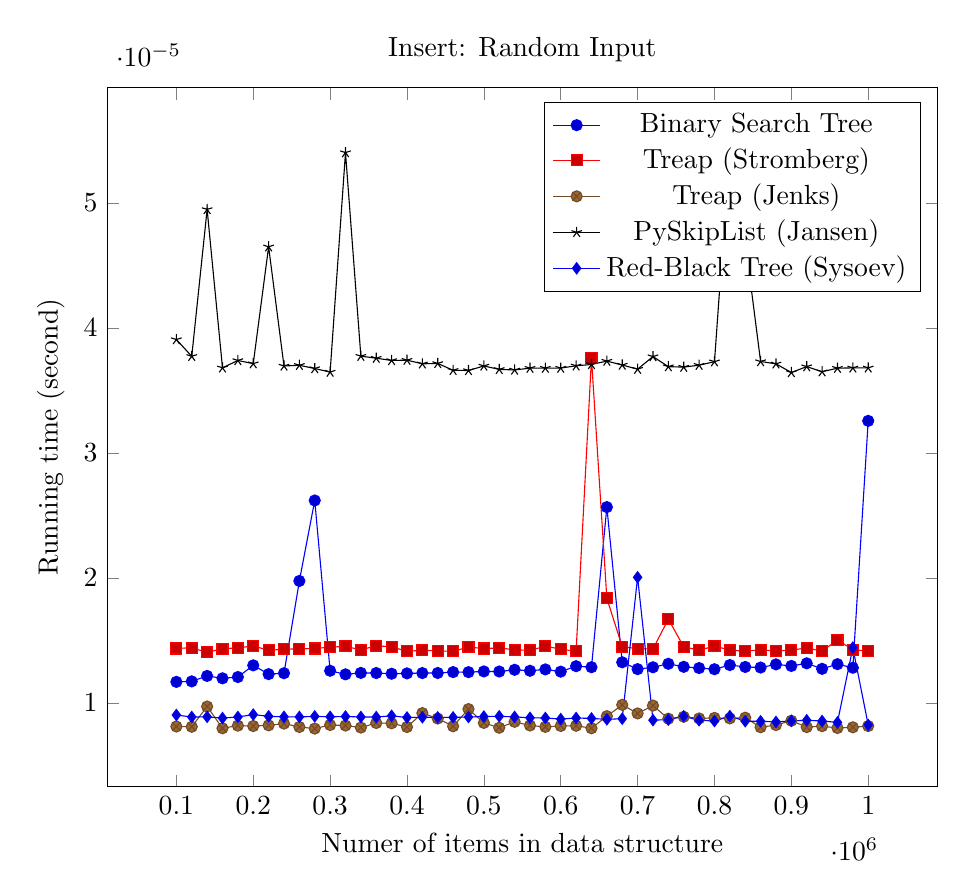
\begin{tikzpicture}
        \begin{axis}[
            xlabel={Numer of items in data structure},
            ylabel={Running time (second)},
            title={Insert: Random Input},
            width=\textwidth
        ]
		\addplot coordinates {
			(100000, 1.1677170156531247e-05)
			(120000, 1.1717527651740057e-05)
			(140000, 1.2152726013255233e-05)
			(160000, 1.1963286726427214e-05)
			(180000, 1.2064180464221862e-05)
			(200000, 1.3000534586240065e-05)
			(220000, 1.2296386648927182e-05)
			(240000, 1.2371078132332514e-05)
			(260000, 1.9754692688252363e-05)
			(280000, 2.619502608933999e-05)
			(300000, 1.2566540925945447e-05)
			(320000, 1.2279219654715234e-05)
			(340000, 1.2394268633329376e-05)
			(360000, 1.2384932197846866e-05)
			(380000, 1.2328010059150074e-05)
			(400000, 1.2357224066931849e-05)
			(420000, 1.238252279529206e-05)
			(440000, 1.2388847477268428e-05)
			(460000, 1.2459021330755605e-05)
			(480000, 1.2456913103392253e-05)
			(500000, 1.2514738768004463e-05)
			(520000, 1.2506607033969886e-05)
			(540000, 1.2644545338162062e-05)
			(560000, 1.2565938575335168e-05)
			(580000, 1.267616874849864e-05)
			(600000, 1.249606589715313e-05)
			(620000, 1.2934276012060763e-05)
			(640000, 1.2851452794620855e-05)
			(660000, 2.5664355145977426e-05)
			(680000, 1.3244787784287837e-05)
			(700000, 1.269755219743729e-05)
			(720000, 1.284603163844622e-05)
			(740000, 1.3124016474307609e-05)
			(760000, 1.2880365626870116e-05)
			(780000, 1.2783989519107308e-05)
			(800000, 1.269032398931813e-05)
			(820000, 1.3023423911818099e-05)
			(840000, 1.2872233892721852e-05)
			(860000, 1.2823443488173325e-05)
			(880000, 1.3077334297122433e-05)
			(900000, 1.2952647707720644e-05)
			(920000, 1.316286809264966e-05)
			(940000, 1.272074269843415e-05)
			(960000, 1.3095404817249801e-05)
			(980000, 1.2808685896743555e-05)
			(1000000, 3.256548681224558e-05)
		};
		\addplot coordinates {
			(100000, 1.4354317724951216e-05)
			(120000, 1.440883046086583e-05)
			(140000, 1.4037180095328949e-05)
			(160000, 1.4332934276012565e-05)
			(180000, 1.4394675220046339e-05)
			(200000, 1.45576110771799e-05)
			(220000, 1.4199513601738546e-05)
			(240000, 1.4293781482251688e-05)
			(260000, 1.4317875509163968e-05)
			(280000, 1.4347691867556022e-05)
			(300000, 1.4458825566748601e-05)
			(320000, 1.451665123136081e-05)
			(340000, 1.4244689902284335e-05)
			(360000, 1.4564236934575092e-05)
			(380000, 1.4485328996329372e-05)
			(400000, 1.4116690384184949e-05)
			(420000, 1.4214572368700829e-05)
			(440000, 1.4156144353364653e-05)
			(460000, 1.4124520943028074e-05)
			(480000, 1.4462138495559884e-05)
			(500000, 1.434437893874474e-05)
			(520000, 1.4391061116043602e-05)
			(540000, 1.4244087551674057e-05)
			(560000, 1.4201320653796757e-05)
			(580000, 1.4529300595540917e-05)
			(600000, 1.429829911228353e-05)
			(620000, 1.4124822118333214e-05)
			(640000, 3.757734559110304e-05)
			(660000, 1.836326263241972e-05)
			(680000, 1.449195485383825e-05)
			(700000, 1.433203074998346e-05)
			(720000, 1.4312755528408161e-05)
			(740000, 1.6702883000903058e-05)
			(760000, 1.4477197262294793e-05)
			(780000, 1.421999352464809e-05)
			(800000, 1.4537131154270355e-05)
			(820000, 1.4227824083491214e-05)
			(840000, 1.4126327994972599e-05)
			(860000, 1.4242882850339811e-05)
			(880000, 1.414921732066432e-05)
			(900000, 1.4219692349456636e-05)
			(920000, 1.4390759940738463e-05)
			(940000, 1.4131749151033547e-05)
			(960000, 1.5036781038020308e-05)
			(980000, 1.4251014584488075e-05)
			(1000000, 1.4142892638574267e-05)
		};
		\addplot coordinates {
			(100000, 8.106736539275516e-06)
			(120000, 8.086858967089937e-06)
			(140000, 9.706278752787512e-06)
			(160000, 7.965485306499432e-06)
			(180000, 8.175103340704482e-06)
			(200000, 8.143479930367903e-06)
			(220000, 8.200402069064694e-06)
			(240000, 8.339243899285975e-06)
			(260000, 8.067282570209499e-06)
			(280000, 7.939885402720392e-06)
			(300000, 8.227507849369431e-06)
			(320000, 8.183235074852746e-06)
			(340000, 8.020299217719184e-06)
			(360000, 8.388937829863608e-06)
			(380000, 8.366349679590712e-06)
			(400000, 8.06427081693073e-06)
			(420000, 9.176812510759191e-06)
			(440000, 8.742216499967981e-06)
			(460000, 8.126312936269642e-06)
			(480000, 9.498768945832126e-06)
			(500000, 8.39496133664852e-06)
			(520000, 8.005842801480868e-06)
			(540000, 8.482001008928819e-06)
			(560000, 8.185343302216098e-06)
			(580000, 8.07631783038687e-06)
			(600000, 8.149804612457956e-06)
			(620000, 8.166068080640798e-06)
			(640000, 7.967593533862782e-06)
			(660000, 8.931053435958347e-06)
			(680000, 9.83879590091874e-06)
			(700000, 9.153019659265737e-06)
			(720000, 9.78066906100139e-06)
			(740000, 8.731675363151225e-06)
			(760000, 8.886780661555349e-06)
			(780000, 8.751854110641943e-06)
			(800000, 8.79130807970796e-06)
			(820000, 8.75305881197619e-06)
			(840000, 8.811486827312365e-06)
			(860000, 8.046802647413642e-06)
			(880000, 8.224496095976974e-06)
			(900000, 8.566330103235486e-06)
			(920000, 8.05764495942185e-06)
			(940000, 8.1335411443888e-06)
			(960000, 7.986567579905568e-06)
			(980000, 8.042285017268113e-06)
			(1000000, 8.142576404452484e-06)
		};
		\addplot coordinates {
			(100000, 3.907388583957072e-05)
			(120000, 3.7732450889507165e-05)
			(140000, 4.948611958161564e-05)
			(160000, 3.6811456709870074e-05)
			(180000, 3.739844744120546e-05)
			(200000, 3.7144556632256356e-05)
			(220000, 4.64969543644429e-05)
			(240000, 3.695782792351565e-05)
			(260000, 3.7014448886793616e-05)
			(280000, 3.675332986983904e-05)
			(300000, 3.647052622864067e-05)
			(320000, 5.4035674218653184e-05)
			(340000, 3.774238967571364e-05)
			(360000, 3.75812608705246e-05)
			(380000, 3.7397845090481495e-05)
			(400000, 3.742344499403316e-05)
			(420000, 3.713220844349507e-05)
			(440000, 3.716292832780255e-05)
			(460000, 3.661268098755954e-05)
			(480000, 3.6596116344071563e-05)
			(500000, 3.6959634975460175e-05)
			(520000, 3.668586659443918e-05)
			(540000, 3.663948559255914e-05)
			(560000, 3.678374857884137e-05)
			(580000, 3.678796503356807e-05)
			(600000, 3.6790073260931425e-05)
			(620000, 3.697017611227693e-05)
			(640000, 3.7079201584219845e-05)
			(660000, 3.734905468593297e-05)
			(680000, 3.703492880970316e-05)
			(700000, 3.670213006262202e-05)
			(720000, 3.771046509007192e-05)
			(740000, 3.690361636290618e-05)
			(760000, 3.686717414711893e-05)
			(780000, 3.7022279445523056e-05)
			(800000, 3.7299661930774166e-05)
			(820000, 5.4553093447225365e-05)
			(840000, 4.693636918068478e-05)
			(860000, 3.7314419522090246e-05)
			(880000, 3.7128895514797476e-05)
			(900000, 3.6437396941551016e-05)
			(920000, 3.690512223954556e-05)
			(940000, 3.649853553497451e-05)
			(960000, 3.6782543877507126e-05)
			(980000, 3.680543320308516e-05)
			(1000000, 3.680964965781186e-05)
		};
		\addplot coordinates {
			(100000, 9.02622484238691e-06)
			(120000, 8.863590160672174e-06)
			(140000, 8.877745401491665e-06)
			(160000, 8.78167046892031e-06)
			(180000, 8.867204264561223e-06)
			(200000, 9.060257655505667e-06)
			(220000, 8.917199370557682e-06)
			(240000, 8.879552453549878e-06)
			(260000, 8.870517193372506e-06)
			(280000, 8.917199370557682e-06)
			(300000, 8.87955245343619e-06)
			(320000, 8.906658233740928e-06)
			(340000, 8.86750543998005e-06)
			(360000, 8.860277231860891e-06)
			(380000, 8.959665093016157e-06)
			(400000, 8.827750295495206e-06)
			(420000, 8.8461219910414e-06)
			(440000, 8.837387906282857e-06)
			(460000, 8.836785555672577e-06)
			(480000, 8.86720426467491e-06)
			(500000, 8.903044129738191e-06)
			(520000, 8.922018175894663e-06)
			(540000, 8.875938349433454e-06)
			(560000, 8.80034333988533e-06)
			(580000, 8.785886923647013e-06)
			(600000, 8.699449602090681e-06)
			(620000, 8.78528457315042e-06)
			(640000, 8.753058812089876e-06)
			(660000, 8.678969679181137e-06)
			(680000, 8.731073012427259e-06)
			(700000, 2.0048338641572627e-05)
			(720000, 8.613915806449767e-06)
			(740000, 8.653972126239751e-06)
			(760000, 8.923825227952876e-06)
			(780000, 8.612108754505244e-06)
			(800000, 8.543139602352311e-06)
			(820000, 8.937378118162087e-06)
			(840000, 8.527779660198576e-06)
			(860000, 8.525671432835225e-06)
			(880000, 8.47176104753089e-06)
			(900000, 8.553078388331414e-06)
			(920000, 8.606085247606642e-06)
			(940000, 8.542537251628346e-06)
			(960000, 8.4383305851361e-06)
			(980000, 1.4417865721043199e-05)
			(1000000, 8.228411375398537e-06)
		};
        \legend{Binary Search Tree, Treap (Stromberg), Treap (Jenks), PySkipList (Jansen), Red-Black Tree (Sysoev)}
        \end{axis}
    \end{tikzpicture}
    \caption{Average of 1000 operations, benchmarked every 20000, starting at 100000.}
\end{figure}
% \begin{figure}[h]
    \centering
    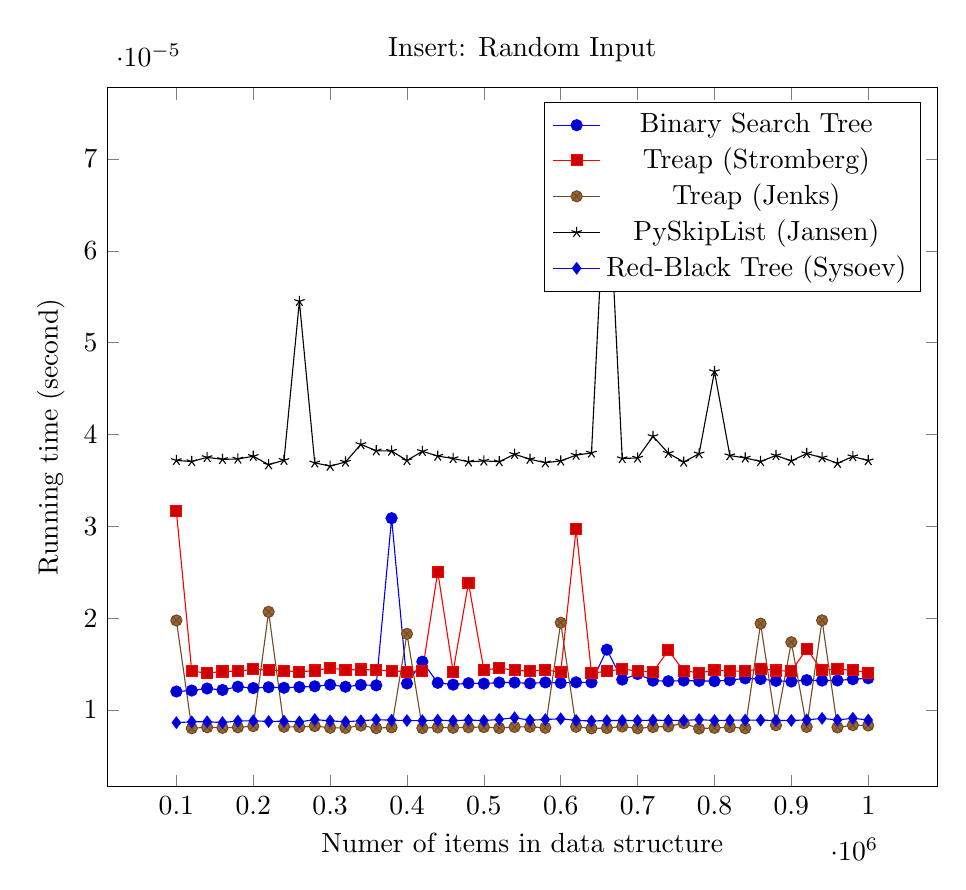
\begin{tikzpicture}
        \begin{axis}[
            xlabel={Numer of items in data structure},
            ylabel={Running time (second)},
            title={Insert: Random Input},
            width=\textwidth
        ]
		\addplot coordinates {
			(100000, 1.2014486533757918e-05)
			(120000, 1.2121403778223794e-05)
			(140000, 1.2342466475388391e-05)
			(160000, 1.2182843546952426e-05)
			(180000, 1.2540037496364675e-05)
			(200000, 1.2390654529212952e-05)
			(220000, 1.2479802428970288e-05)
			(240000, 1.2420772063023834e-05)
			(260000, 1.2498174124516482e-05)
			(280000, 1.2581599692794044e-05)
			(300000, 1.2756281388078605e-05)
			(320000, 1.2535218690914007e-05)
			(340000, 1.273068148452694e-05)
			(360000, 1.2681891079978413e-05)
			(380000, 3.088643430999127e-05)
			(400000, 1.2883979730872853e-05)
			(420000, 1.5265975469219482e-05)
			(440000, 1.2960478266450082e-05)
			(460000, 1.2763810771502903e-05)
			(480000, 1.2923132524747417e-05)
			(500000, 1.2873739769361237e-05)
			(520000, 1.299210167678666e-05)
			(540000, 1.2994209904150012e-05)
			(560000, 1.2898737322416309e-05)
			(580000, 1.3006256917606151e-05)
			(600000, 1.294692537624087e-05)
			(620000, 1.3018605106367431e-05)
			(640000, 1.3012280424391065e-05)
			(660000, 1.6572172904716352e-05)
			(680000, 1.3310745183048312e-05)
			(700000, 1.3920022889351458e-05)
			(720000, 1.3198406782521488e-05)
			(740000, 1.3140279942490451e-05)
			(760000, 1.3206237341250926e-05)
			(780000, 1.3170999826797925e-05)
			(800000, 1.3141183468519557e-05)
			(820000, 1.325081129107275e-05)
			(840000, 1.3447779961211382e-05)
			(860000, 1.3372486127195771e-05)
			(880000, 1.3171301002103064e-05)
			(900000, 1.3103837726816891e-05)
			(920000, 1.3256533622552524e-05)
			(940000, 1.320322558785847e-05)
			(960000, 1.32176820039831e-05)
			(980000, 1.3356825009623208e-05)
			(1000000, 1.3459224624057242e-05)
		};
		\addplot coordinates {
			(100000, 3.163816795051844e-05)
			(120000, 1.4234449940886406e-05)
			(140000, 1.4013688419026948e-05)
			(160000, 1.4203428881273794e-05)
			(180000, 1.4227522908072387e-05)
			(200000, 1.4431117435833584e-05)
			(220000, 1.4346487166221778e-05)
			(240000, 1.4275409786705496e-05)
			(260000, 1.4157951405309177e-05)
			(280000, 1.4296793235644145e-05)
			(300000, 1.456393575938364e-05)
			(320000, 1.4371484719049477e-05)
			(340000, 1.4405216356749406e-05)
			(360000, 1.4354317724837529e-05)
			(380000, 1.4267579227976058e-05)
			(400000, 1.4180539555582072e-05)
			(420000, 1.4205838283942284e-05)
			(440000, 2.5053270387729753e-05)
			(460000, 1.418325013366939e-05)
			(480000, 2.3838630254545023e-05)
			(500000, 1.4345282464773845e-05)
			(520000, 1.455730990187476e-05)
			(540000, 1.4337150730739268e-05)
			(560000, 1.4226318206738142e-05)
			(580000, 1.436485886176797e-05)
			(600000, 1.412572564436232e-05)
			(620000, 2.973293277011635e-05)
			(640000, 1.4020314276422142e-05)
			(660000, 1.421637942075904e-05)
			(680000, 1.4460331443387986e-05)
			(700000, 1.4237762869584002e-05)
			(720000, 1.4153734950696162e-05)
			(740000, 1.6492963791165495e-05)
			(760000, 1.4276313312734601e-05)
			(780000, 1.405163651145358e-05)
			(800000, 1.4313960229742406e-05)
			(820000, 1.4260652195162038e-05)
			(840000, 1.4206741809857704e-05)
			(860000, 1.450249599054132e-05)
			(880000, 1.4302214391705093e-05)
			(900000, 1.4214572368700829e-05)
			(920000, 1.6654694947078497e-05)
			(940000, 1.431968256122218e-05)
			(960000, 1.4447983254626706e-05)
			(980000, 1.4313960229856093e-05)
			(1000000, 1.4068803505665528e-05)
		};
		\addplot coordinates {
			(100000, 1.9755596214281467e-05)
			(120000, 8.013071009600026e-06)
			(140000, 8.120289429484728e-06)
			(160000, 8.059150836061235e-06)
			(180000, 8.112157695450151e-06)
			(200000, 8.238651336796465e-06)
			(220000, 2.069285386221509e-05)
			(240000, 8.176609217457554e-06)
			(260000, 8.157635171187394e-06)
			(280000, 8.248288947584114e-06)
			(300000, 8.06969197287799e-06)
			(320000, 8.049513225387272e-06)
			(340000, 8.30912636558878e-06)
			(360000, 8.026322724390411e-06)
			(380000, 8.10553183794127e-06)
			(400000, 1.829579935701986e-05)
			(420000, 8.027828601143483e-06)
			(440000, 8.105833013360098e-06)
			(460000, 8.06517434284615e-06)
			(480000, 8.119687078874448e-06)
			(500000, 8.137456423696676e-06)
			(520000, 8.038369737960238e-06)
			(540000, 8.153418716460692e-06)
			(560000, 8.166971606669904e-06)
			(580000, 8.065776693570114e-06)
			(600000, 1.9508030087422412e-05)
			(620000, 8.17058571067264e-06)
			(640000, 7.99710871683601e-06)
			(660000, 8.03355093250957e-06)
			(680000, 8.200100893759555e-06)
			(700000, 8.007348678233938e-06)
			(720000, 8.141070527699412e-06)
			(740000, 8.21064203057631e-06)
			(760000, 8.56030659656426e-06)
			(780000, 7.979038196594956e-06)
			(800000, 8.051019102026657e-06)
			(820000, 8.130529390996343e-06)
			(840000, 8.014576886353098e-06)
			(860000, 1.941255750568871e-05)
			(880000, 8.339243899285975e-06)
			(900000, 1.738293691130366e-05)
			(920000, 8.154623417908624e-06)
			(940000, 1.976433029904001e-05)
			(960000, 8.106736539275516e-06)
			(980000, 8.35008621140787e-06)
			(1000000, 8.313342820315484e-06)
		};
		\addplot coordinates {
			(100000, 3.718370942601723e-05)
			(120000, 3.706233576531304e-05)
			(140000, 3.751108701703742e-05)
			(160000, 3.729785487860227e-05)
			(180000, 3.7340621776479565e-05)
			(200000, 3.763366537907586e-05)
			(220000, 3.671628530344151e-05)
			(240000, 3.719756349153158e-05)
			(260000, 5.450851949728985e-05)
			(280000, 3.691867512964109e-05)
			(300000, 3.655877060225521e-05)
			(320000, 3.7007521854093284e-05)
			(340000, 3.89254063984481e-05)
			(360000, 3.823661840340264e-05)
			(380000, 3.820409146692327e-05)
			(400000, 3.7174975341258686e-05)
			(420000, 3.817427510864491e-05)
			(440000, 3.765324177606999e-05)
			(460000, 3.7396339213842114e-05)
			(480000, 3.702920647822339e-05)
			(500000, 3.712467906007077e-05)
			(520000, 3.704426524518567e-05)
			(540000, 3.7854125725630184e-05)
			(560000, 3.7310203067477235e-05)
			(580000, 3.692951744187667e-05)
			(600000, 3.712618493671016e-05)
			(620000, 3.775654491653313e-05)
			(640000, 3.799356990657543e-05)
			(660000, 7.141017822050344e-05)
			(680000, 3.7391520408391444e-05)
			(700000, 3.744814137166941e-05)
			(720000, 3.980363368043527e-05)
			(740000, 3.7969174704244325e-05)
			(760000, 3.7005413626729936e-05)
			(780000, 3.7911650214937255e-05)
			(800000, 4.686679767792157e-05)
			(820000, 3.770835686259488e-05)
			(840000, 3.7453863703149184e-05)
			(860000, 3.7063540466760966e-05)
			(880000, 3.771769329807739e-05)
			(900000, 3.7130100216131724e-05)
			(920000, 3.793243131326562e-05)
			(940000, 3.747886125609057e-05)
			(960000, 3.687139060173195e-05)
			(980000, 3.760324667018722e-05)
			(1000000, 3.7165638905889864e-05)
		};
		\addplot coordinates {
			(100000, 8.618734611786748e-06)
			(120000, 8.71842364836084e-06)
			(140000, 8.721134226334471e-06)
			(160000, 8.634094553940485e-06)
			(180000, 8.802150391829855e-06)
			(200000, 8.833472626974981e-06)
			(220000, 8.747336480610101e-06)
			(240000, 8.78829632642919e-06)
			(260000, 8.702762530788277e-06)
			(280000, 8.959363917597329e-06)
			(300000, 8.817510334097278e-06)
			(320000, 8.722640103087543e-06)
			(340000, 8.831665574916769e-06)
			(360000, 8.94611220292063e-06)
			(380000, 8.895815921619033e-06)
			(400000, 8.853350199160559e-06)
			(420000, 8.84551964043112e-06)
			(440000, 8.899731201040595e-06)
			(460000, 8.83678555555889e-06)
			(480000, 8.913886441860086e-06)
			(500000, 8.844616114402015e-06)
			(520000, 8.978639139286315e-06)
			(540000, 9.160850217995176e-06)
			(560000, 8.890997116168365e-06)
			(580000, 8.964483898466825e-06)
			(600000, 9.043693011903996e-06)
			(620000, 8.867204264561223e-06)
			(640000, 8.806969197280523e-06)
			(660000, 8.847929043099611e-06)
			(680000, 8.860879582584858e-06)
			(700000, 8.856361952553016e-06)
			(720000, 8.891298291587191e-06)
			(740000, 8.868710141314296e-06)
			(760000, 8.864192511282454e-06)
			(780000, 8.958761567100736e-06)
			(800000, 8.851241971797209e-06)
			(820000, 8.885274784802277e-06)
			(840000, 8.908164110493998e-06)
			(860000, 8.894310044979648e-06)
			(880000, 8.863891335863628e-06)
			(900000, 8.85847017980268e-06)
			(920000, 8.922018175894663e-06)
			(940000, 9.087965786420682e-06)
			(960000, 8.915994669223438e-06)
			(980000, 9.103626903993245e-06)
			(1000000, 8.907862935075172e-06)
		};
        \legend{Binary Search Tree, Treap (Stromberg), Treap (Jenks), PySkipList (Jansen), Red-Black Tree (Sysoev)}
        \end{axis}
    \end{tikzpicture}
    \caption{Average of 1000 operations, benchmarked every 20000, starting at 100000.}
\end{figure}
% \begin{figure}[h]
    \centering
    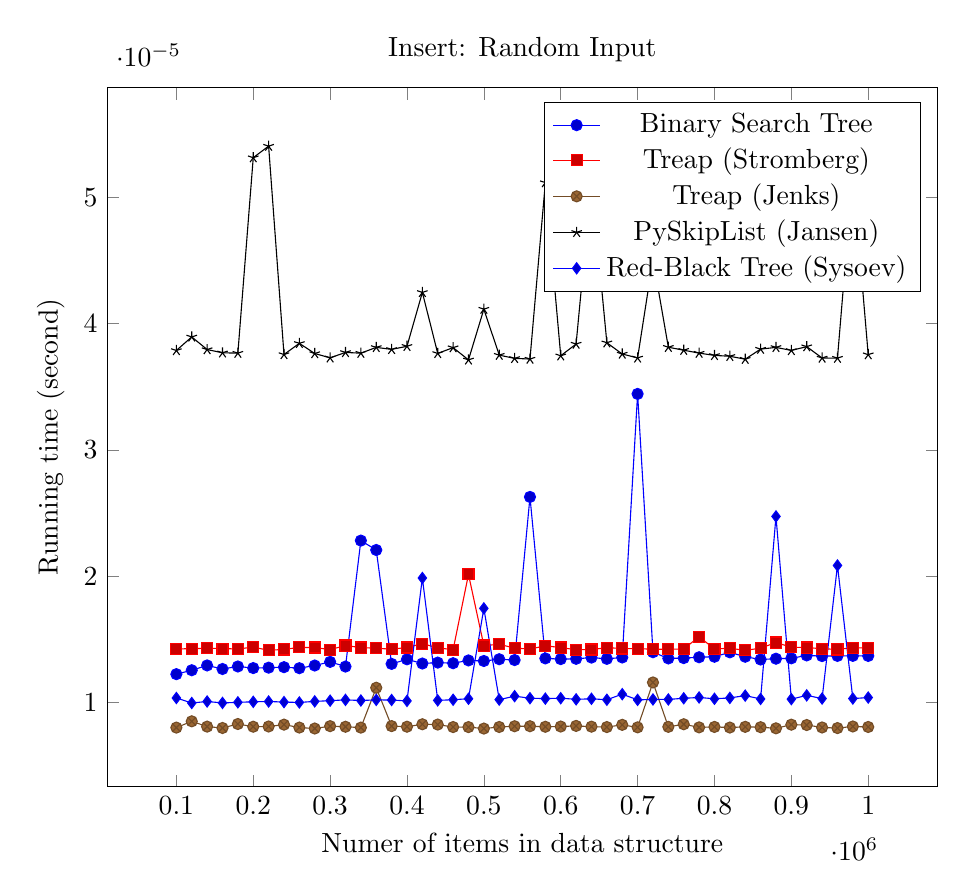
\begin{tikzpicture}
        \begin{axis}[
            xlabel={Numer of items in data structure},
            ylabel={Running time (second)},
            title={Insert: Random Input},
            width=\textwidth
        ]
		\addplot coordinates {
			(100000, 1.2243078614233127e-05)
			(120000, 1.25535903864602e-05)
			(140000, 1.2933673661450484e-05)
			(160000, 1.265147237097608e-05)
			(180000, 1.2850549268478062e-05)
			(200000, 1.2724356802436887e-05)
			(220000, 1.2756883738802572e-05)
			(240000, 1.2796638883287414e-05)
			(260000, 1.2715622717678344e-05)
			(280000, 1.2927650154779257e-05)
			(300000, 1.3214670250590644e-05)
			(320000, 1.2843321060358904e-05)
			(340000, 2.2818850564362948e-05)
			(360000, 2.207494748256522e-05)
			(380000, 1.305655319890775e-05)
			(400000, 1.341856595365698e-05)
			(420000, 1.3084863680546732e-05)
			(440000, 1.315774811200754e-05)
			(460000, 1.3109861233488118e-05)
			(480000, 1.3330321580042437e-05)
			(500000, 1.3285747630220613e-05)
			(520000, 1.3425191811052174e-05)
			(540000, 1.335893323698656e-05)
			(560000, 2.627664460555934e-05)
			(580000, 1.3490848034393821e-05)
			(600000, 1.3433925895810717e-05)
			(620000, 1.3457116396693892e-05)
			(640000, 1.3554094855180665e-05)
			(660000, 1.3454405818720261e-05)
			(680000, 1.3563732465968314e-05)
			(700000, 3.443488212758439e-05)
			(720000, 1.3981763833271543e-05)
			(740000, 1.3487836281115051e-05)
			(760000, 1.3515243236724928e-05)
			(780000, 1.3581501810904229e-05)
			(800000, 1.3621558130694211e-05)
			(820000, 1.397001799523423e-05)
			(840000, 1.3621558130580524e-05)
			(860000, 1.3402603660779278e-05)
			(880000, 1.3466151656871261e-05)
			(900000, 1.3497775067094154e-05)
			(920000, 1.3726969498520702e-05)
			(940000, 1.3673360288521508e-05)
			(960000, 1.3689021405980384e-05)
			(980000, 1.3691129633343736e-05)
			(1000000, 1.3687214354035858e-05)
		};
		\addplot coordinates {
			(100000, 1.4245593428313442e-05)
			(120000, 1.425523103910109e-05)
			(140000, 1.429829911228353e-05)
			(160000, 1.426486864988874e-05)
			(180000, 1.4239268746223387e-05)
			(200000, 1.4382327031171372e-05)
			(220000, 1.4131447975728406e-05)
			(240000, 1.4201621829215583e-05)
			(260000, 1.4360943582346408e-05)
			(280000, 1.4352510672893005e-05)
			(300000, 1.4186261886948159e-05)
			(320000, 1.4507917146602267e-05)
			(340000, 1.4348294218166302e-05)
			(360000, 1.4294986183585934e-05)
			(380000, 1.4221198226096021e-05)
			(400000, 1.4352209497587864e-05)
			(420000, 1.465790246436427e-05)
			(440000, 1.4327814295256758e-05)
			(460000, 1.4177226626884476e-05)
			(480000, 2.0142305346666945e-05)
			(500000, 1.4507013620686849e-05)
			(520000, 1.4605497955813007e-05)
			(540000, 1.4305527320402688e-05)
			(560000, 1.4229631135549425e-05)
			(580000, 1.448954545116976e-05)
			(600000, 1.4348294218166302e-05)
			(620000, 1.4173311347462914e-05)
			(640000, 1.4194393621096424e-05)
			(660000, 1.4336849555434127e-05)
			(680000, 1.427902389070823e-05)
			(700000, 1.4256134565243883e-05)
			(720000, 1.4224511154793617e-05)
			(740000, 1.4209151212639882e-05)
			(760000, 1.424017227236618e-05)
			(780000, 1.5206342752549062e-05)
			(800000, 1.4234148765581267e-05)
			(820000, 1.429588970961504e-05)
			(840000, 1.4124219767722935e-05)
			(860000, 1.4303720268344477e-05)
			(880000, 1.4745544487368535e-05)
			(900000, 1.437479764786076e-05)
			(920000, 1.4347390692137196e-05)
			(940000, 1.4260049844438072e-05)
			(960000, 1.4201320653910444e-05)
			(980000, 1.4337451906044407e-05)
			(1000000, 1.4312755528521849e-05)
		};
		\addplot coordinates {
			(100000, 8.010360431626395e-06)
			(120000, 8.507600912594171e-06)
			(140000, 8.08836484384301e-06)
			(160000, 7.979941722510375e-06)
			(180000, 8.295573475493256e-06)
			(200000, 8.080534285113572e-06)
			(220000, 8.098303629935799e-06)
			(240000, 8.246180720220764e-06)
			(260000, 8.013372185018852e-06)
			(280000, 7.938078350775869e-06)
			(300000, 8.126011760850816e-06)
			(320000, 8.077221356302289e-06)
			(340000, 8.008854554873323e-06)
			(360000, 1.116607561004912e-05)
			(380000, 8.128119988214166e-06)
			(400000, 8.080835460418712e-06)
			(420000, 8.274491201859746e-06)
			(440000, 8.251601876281712e-06)
			(460000, 8.053729680113975e-06)
			(480000, 8.050416751416379e-06)
			(500000, 7.9332595453252e-06)
			(520000, 8.059452011480061e-06)
			(540000, 8.117880026816237e-06)
			(560000, 8.120289429484728e-06)
			(580000, 8.076317830273183e-06)
			(600000, 8.094990701124516e-06)
			(620000, 8.144684631702149e-06)
			(640000, 8.084750739726588e-06)
			(660000, 8.05222380347459e-06)
			(680000, 8.229616076732781e-06)
			(700000, 8.029936828506833e-06)
			(720000, 1.1585612854219108e-05)
			(740000, 8.069390797686538e-06)
			(760000, 8.275997078612818e-06)
			(780000, 8.028129776448622e-06)
			(800000, 8.063066115482798e-06)
			(820000, 8.014878061658237e-06)
			(840000, 8.070896674212236e-06)
			(860000, 8.041682666544148e-06)
			(880000, 7.953137117624465e-06)
			(900000, 8.243470142133446e-06)
			(920000, 8.21365378385508e-06)
			(940000, 8.020600393024323e-06)
			(960000, 7.972713514504903e-06)
			(980000, 8.099508331270045e-06)
			(1000000, 8.059753186785202e-06)
		};
		\addplot coordinates {
			(100000, 3.7875810349873974e-05)
			(120000, 3.894678984738675e-05)
			(140000, 3.794899595663992e-05)
			(160000, 3.769149104380176e-05)
			(180000, 3.766378291277306e-05)
			(200000, 5.3141484643788315e-05)
			(220000, 5.405826236892608e-05)
			(240000, 3.7556263317583217e-05)
			(260000, 3.8439309404907364e-05)
			(280000, 3.763306302846559e-05)
			(300000, 3.729303607326528e-05)
			(320000, 3.771889799941164e-05)
			(340000, 3.7662578211552497e-05)
			(360000, 3.8119160022006326e-05)
			(380000, 3.7960741794904604e-05)
			(400000, 3.820710322031573e-05)
			(420000, 4.247385421615491e-05)
			(440000, 3.7642700639253236e-05)
			(460000, 3.810108950176527e-05)
			(480000, 3.713100374216083e-05)
			(500000, 4.114747803305363e-05)
			(520000, 3.750536468567134e-05)
			(540000, 3.725026917550167e-05)
			(560000, 3.719605761477851e-05)
			(580000, 5.11690873634052e-05)
			(600000, 3.7456574281122814e-05)
			(620000, 3.838630254574582e-05)
			(640000, 5.126727052322622e-05)
			(660000, 3.8486593932816506e-05)
			(680000, 3.759601846206806e-05)
			(700000, 3.728460316392557e-05)
			(720000, 4.511817367279036e-05)
			(740000, 3.8132110561491576e-05)
			(760000, 3.7895687922173235e-05)
			(780000, 3.76658911402501e-05)
			(800000, 3.74857882887909e-05)
			(820000, 3.741561443530372e-05)
			(840000, 3.7185516477961755e-05)
			(860000, 3.7982125243843254e-05)
			(880000, 3.812006354803543e-05)
			(900000, 3.787731622662705e-05)
			(920000, 3.8179093913981885e-05)
			(940000, 3.727918200775093e-05)
			(960000, 3.726833969562904e-05)
			(980000, 5.189883520449712e-05)
			(1000000, 3.7544818654737355e-05)
		};
		\addplot coordinates {
			(100000, 1.0355010428270362e-05)
			(120000, 9.958362509678409e-06)
			(140000, 1.0078832644353498e-05)
			(160000, 9.962578964405112e-06)
			(180000, 1.0011369369067324e-05)
			(200000, 1.0053533916106971e-05)
			(220000, 1.0078531469048357e-05)
			(240000, 1.0032752817892288e-05)
			(260000, 1.0001731758165988e-05)
			(280000, 1.0086663203196623e-05)
			(300000, 1.014238064044548e-05)
			(320000, 1.0206530987147743e-05)
			(340000, 1.0155933530541007e-05)
			(360000, 1.0205025110508358e-05)
			(380000, 1.0194182798386465e-05)
			(400000, 1.012159954211711e-05)
			(420000, 1.985558642604701e-05)
			(440000, 1.0165872316633794e-05)
			(460000, 1.0217674474688466e-05)
			(480000, 1.0295377711486253e-05)
			(500000, 1.7452809589485696e-05)
			(520000, 1.0224601507388798e-05)
			(540000, 1.0498369888523485e-05)
			(560000, 1.0338144609249866e-05)
			(580000, 1.0306220023608148e-05)
			(600000, 1.0339650486002938e-05)
			(620000, 1.0249900235635323e-05)
			(640000, 1.0290860081454412e-05)
			(660000, 1.0214963896601148e-05)
			(680000, 1.065829399226459e-05)
			(700000, 1.020743451317685e-05)
			(720000, 1.02405638002665e-05)
			(740000, 1.0240262624847674e-05)
			(760000, 1.0333325803912885e-05)
			(780000, 1.0395367923365483e-05)
			(800000, 1.0294173010152008e-05)
			(820000, 1.0360431584217622e-05)
			(840000, 1.0544148539679554e-05)
			(860000, 1.0280921295247936e-05)
			(880000, 2.4734325706049277e-05)
			(900000, 1.0263453125730847e-05)
			(920000, 1.0562520235225748e-05)
			(940000, 1.0308629426276638e-05)
			(960000, 2.08536814919853e-05)
			(980000, 1.0308930601695466e-05)
			(1000000, 1.0389946767304537e-05)
		};
        \legend{Binary Search Tree, Treap (Stromberg), Treap (Jenks), PySkipList (Jansen), Red-Black Tree (Sysoev)}
        \end{axis}
    \end{tikzpicture}
    \caption{Average of 1000 operations, benchmarked every 20000, starting at 100000.}
\end{figure}
% \begin{figure}[h]
    \centering
    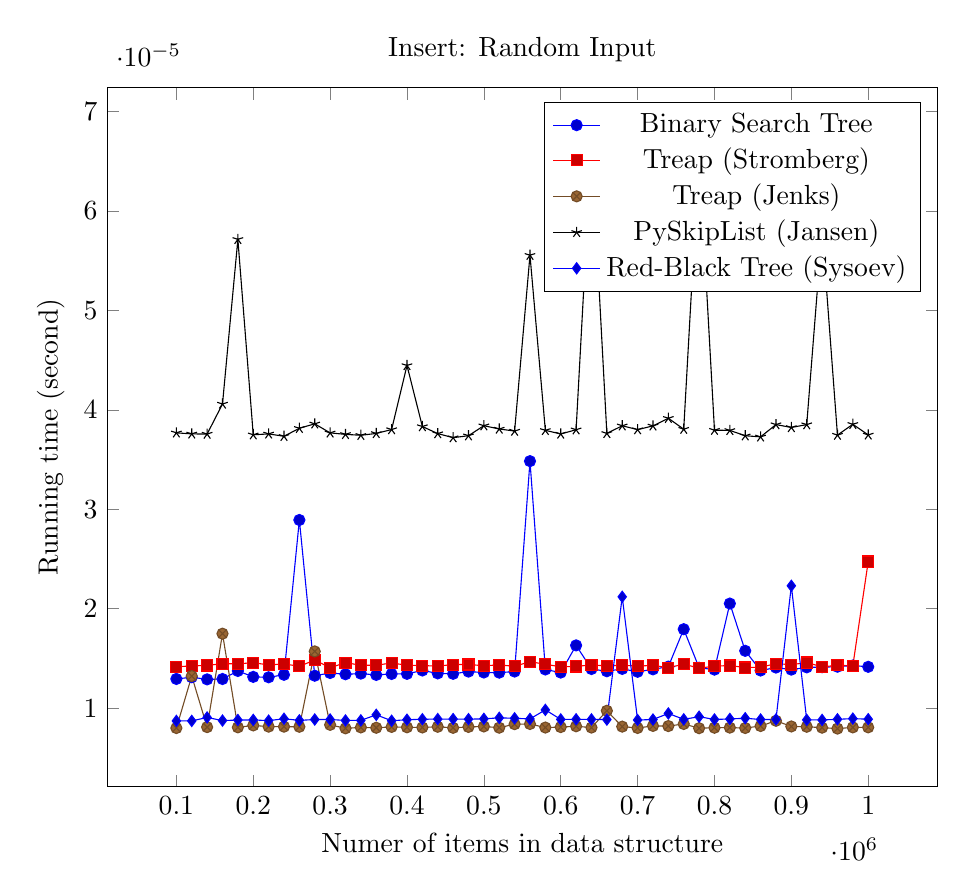
\begin{tikzpicture}
        \begin{axis}[
            xlabel={Numer of items in data structure},
            ylabel={Running time (second)},
            title={Insert: Random Input},
            width=\textwidth
        ]
		\addplot coordinates {
			(100000, 1.29439136229621e-05)
			(120000, 1.3118896493665489e-05)
			(140000, 1.29011467250848e-05)
			(160000, 1.293728776545322e-05)
			(180000, 1.374714824601142e-05)
			(200000, 1.3152025780641452e-05)
			(220000, 1.3111668285432643e-05)
			(240000, 1.3362848516294435e-05)
			(260000, 2.8926385218255746e-05)
			(280000, 1.3268580636008665e-05)
			(300000, 1.354325254305877e-05)
			(320000, 1.3415855375569664e-05)
			(340000, 1.3480005722271926e-05)
			(360000, 1.3350500327533155e-05)
			(380000, 1.3447177610601103e-05)
			(400000, 1.3456514046083612e-05)
			(420000, 1.3795035124644529e-05)
			(440000, 1.3503497398573927e-05)
			(460000, 1.3459525799476068e-05)
			(480000, 1.3682094373280052e-05)
			(500000, 1.3592946473522716e-05)
			(520000, 1.357668300545356e-05)
			(540000, 1.368661200342558e-05)
			(560000, 3.484478176085304e-05)
			(580000, 1.3895627687020351e-05)
			(600000, 1.3584814739488138e-05)
			(620000, 1.6319486797215176e-05)
			(640000, 1.3943213390234633e-05)
			(660000, 1.3717934238343332e-05)
			(680000, 1.3954055702356528e-05)
			(700000, 1.3663722677733858e-05)
			(720000, 1.3909180577229563e-05)
			(740000, 1.418565953633788e-05)
			(760000, 1.794824301839526e-05)
			(780000, 1.4067297628912456e-05)
			(800000, 1.3879966569561476e-05)
			(820000, 2.052449684890689e-05)
			(840000, 1.5771046509030383e-05)
			(860000, 1.3791119845222966e-05)
			(880000, 1.4087777551935687e-05)
			(900000, 1.3882677147535105e-05)
			(920000, 1.4110064526789757e-05)
			(940000, 1.412783387172567e-05)
			(960000, 1.4175118399634812e-05)
			(980000, 1.4295889709501352e-05)
			(1000000, 1.4163071386064985e-05)
		};
		\addplot coordinates {
			(100000, 1.4165480788847163e-05)
			(120000, 1.4255231039214778e-05)
			(140000, 1.4304021443763303e-05)
			(160000, 1.4483823119689987e-05)
			(180000, 1.4456114988661285e-05)
			(200000, 1.4584716857484636e-05)
			(220000, 1.4349498919500548e-05)
			(240000, 1.4459427917472568e-05)
			(260000, 1.4214271193282001e-05)
			(280000, 1.4846739400468322e-05)
			(300000, 1.4070008206999773e-05)
			(320000, 1.457899452611855e-05)
			(340000, 1.432239313919581e-05)
			(360000, 1.4325706067893406e-05)
			(380000, 1.454737111578197e-05)
			(400000, 1.4325404892588267e-05)
			(420000, 1.4283541520740073e-05)
			(440000, 1.4241979324310705e-05)
			(460000, 1.4387447011927178e-05)
			(480000, 1.4397988148743934e-05)
			(500000, 1.4274205085257563e-05)
			(520000, 1.4352209497587864e-05)
			(540000, 1.4216379420645353e-05)
			(560000, 1.4675972984491636e-05)
			(580000, 1.4419371597682584e-05)
			(600000, 1.416457726270437e-05)
			(620000, 1.4201621829101896e-05)
			(640000, 1.4359437705707023e-05)
			(660000, 1.4247099304952827e-05)
			(680000, 1.433203074998346e-05)
			(700000, 1.4225715856127863e-05)
			(720000, 1.4317875509163968e-05)
			(740000, 1.4067899979636423e-05)
			(760000, 1.4436839767199672e-05)
			(780000, 1.4029048361294372e-05)
			(800000, 1.4229631135549425e-05)
			(820000, 1.4291673254888338e-05)
			(840000, 1.4092596357272668e-05)
			(860000, 1.4115485682964391e-05)
			(880000, 1.4483521944384848e-05)
			(900000, 1.4379917628502881e-05)
			(920000, 1.4589836838240444e-05)
			(940000, 1.4163372561370124e-05)
			(960000, 1.4309442599824251e-05)
			(980000, 1.4273301559342144e-05)
			(1000000, 2.4748782122173908e-05)
		};
		\addplot coordinates {
			(100000, 8.008553379568184e-06)
			(120000, 1.3231536069497451e-05)
			(140000, 8.101315383328256e-06)
			(160000, 1.7496178837859587e-05)
			(180000, 8.077522531721115e-06)
			(200000, 8.272081799191255e-06)
			(220000, 8.149503437266504e-06)
			(240000, 8.146190508455219e-06)
			(260000, 8.135348196333326e-06)
			(280000, 1.5715027896362698e-05)
			(300000, 8.329907463917152e-06)
			(320000, 7.97813467056585e-06)
			(340000, 8.070294323601956e-06)
			(360000, 8.035659159872921e-06)
			(380000, 8.12239765684808e-06)
			(400000, 8.083546038392342e-06)
			(420000, 8.066077868875255e-06)
			(440000, 8.13414349499908e-06)
			(460000, 8.028430951753763e-06)
			(480000, 8.119687078760763e-06)
			(500000, 8.166670431364765e-06)
			(520000, 8.041983841962974e-06)
			(540000, 8.39797308992729e-06)
			(560000, 8.4148389088341e-06)
			(580000, 8.057343784116711e-06)
			(600000, 8.10342361057792e-06)
			(620000, 8.185945652826377e-06)
			(640000, 8.05463320614308e-06)
			(660000, 9.74452802063297e-06)
			(680000, 8.150105787763096e-06)
			(700000, 8.014878061658237e-06)
			(720000, 8.221484342584517e-06)
			(740000, 8.205522049820502e-06)
			(760000, 8.41694713619745e-06)
			(780000, 7.992591086690482e-06)
			(800000, 8.038068562655099e-06)
			(820000, 8.048609699358166e-06)
			(840000, 8.010360431626395e-06)
			(860000, 8.211244381186589e-06)
			(880000, 8.73619299306938e-06)
			(900000, 8.166670431364765e-06)
			(920000, 8.13595054705729e-06)
			(940000, 8.044995595355431e-06)
			(960000, 7.952534766900498e-06)
			(980000, 8.07390842771838e-06)
			(1000000, 8.077221356415976e-06)
		};
		\addplot coordinates {
			(100000, 3.769118986849662e-05)
			(120000, 3.7585477325251306e-05)
			(140000, 3.756800915573422e-05)
			(160000, 4.0592411887473646e-05)
			(180000, 5.714741779797805e-05)
			(200000, 3.749723295163676e-05)
			(220000, 3.7582766747163984e-05)
			(240000, 3.7345741757235376e-05)
			(260000, 3.815018108173263e-05)
			(280000, 3.8596824106093664e-05)
			(300000, 3.7686069887740815e-05)
			(320000, 3.7536686920702775e-05)
			(340000, 3.744603314430606e-05)
			(360000, 3.763005127518682e-05)
			(380000, 3.802218156363324e-05)
			(400000, 4.4464322016665394e-05)
			(420000, 3.832606747835143e-05)
			(440000, 3.761559485883481e-05)
			(460000, 3.720539405037471e-05)
			(480000, 3.740176036978937e-05)
			(500000, 3.840858952059989e-05)
			(520000, 3.8078200176187235e-05)
			(540000, 3.786918449247878e-05)
			(560000, 5.555028498713455e-05)
			(580000, 3.794116539802417e-05)
			(600000, 3.75770444157979e-05)
			(620000, 3.800230399133398e-05)
			(640000, 6.652119897910325e-05)
			(660000, 3.763366537907586e-05)
			(680000, 3.840136131259442e-05)
			(700000, 3.8012543952731905e-05)
			(720000, 3.838931429902459e-05)
			(740000, 3.91573114077346e-05)
			(760000, 3.80586237793068e-05)
			(780000, 6.571103732312622e-05)
			(800000, 3.795893474273271e-05)
			(820000, 3.79363465925735e-05)
			(840000, 3.7398447441091777e-05)
			(860000, 3.728610904056495e-05)
			(880000, 3.852002439521129e-05)
			(900000, 3.823240194856225e-05)
			(920000, 3.8516711466513696e-05)
			(940000, 5.812864704512321e-05)
			(960000, 3.7462898963212865e-05)
			(980000, 3.8551346630242736e-05)
			(1000000, 3.748247536009331e-05)
		};
		\addplot coordinates {
			(100000, 8.723543629002961e-06)
			(120000, 8.725651856366313e-06)
			(140000, 9.072003493656667e-06)
			(160000, 8.756974091397752e-06)
			(180000, 8.812992704065436e-06)
			(200000, 8.825340892826716e-06)
			(220000, 8.751251759917977e-06)
			(240000, 8.940389871440857e-06)
			(260000, 8.779562241670647e-06)
			(280000, 8.863590160558487e-06)
			(300000, 8.86750543998005e-06)
			(320000, 8.770828156912102e-06)
			(340000, 8.778357540336401e-06)
			(360000, 9.337037790032809e-06)
			(380000, 8.740409447909769e-06)
			(400000, 8.84431493898319e-06)
			(420000, 8.890394765558085e-06)
			(440000, 8.907260584351206e-06)
			(460000, 8.907561759770033e-06)
			(480000, 8.899430025621768e-06)
			(500000, 8.932258137292593e-06)
			(520000, 9.03224834928551e-06)
			(540000, 8.98978262671335e-06)
			(560000, 8.92231935131349e-06)
			(580000, 9.83638649825025e-06)
			(600000, 8.876239524738595e-06)
			(620000, 8.888286538194734e-06)
			(640000, 8.879853628855016e-06)
			(660000, 8.858169004611227e-06)
			(680000, 2.120364723327839e-05)
			(700000, 8.81299270395175e-06)
			(720000, 8.8653972126167e-06)
			(740000, 9.472566691442807e-06)
			(760000, 8.883467732857753e-06)
			(780000, 9.148803204539035e-06)
			(800000, 8.870517193372506e-06)
			(820000, 8.920512299255278e-06)
			(840000, 8.993697906021225e-06)
			(860000, 8.866903089369772e-06)
			(880000, 8.870818368677647e-06)
			(900000, 2.2313478349246906e-05)
			(920000, 8.83196675022191e-06)
			(940000, 8.822931490158225e-06)
			(960000, 8.883467732744066e-06)
			(980000, 8.95846039168191e-06)
			(1000000, 8.892502992921435e-06)
		};
        \legend{Binary Search Tree, Treap (Stromberg), Treap (Jenks), PySkipList (Jansen), Red-Black Tree (Sysoev)}
        \end{axis}
    \end{tikzpicture}
    \caption{Average of 1000 operations, benchmarked every 20000, starting at 100000.}
\end{figure}

\end{document}
